\chapter{The mesoSPIM Microscope} 

The aim of this chapter is to introduce the mesoSPIM microscope and its associated protocols utilized to record and process structural, volumetric images of cardiac tissue. The design and operation of the mesoSPIM system essential to achieve peak performance in the imaging pipeline are explained here in detail along with those imaging protocols implemented with the system's control software. Further to this, in this chapter, data processing and storage protocols were implemented. These protocols demonstrate an efficient and reliable means by which the multiple terabytes of data recorded by the mesoSPIM hardware can be managed. When combined, these mesoSPIM hardware and software based protocols provide the high imaging throughput and quality essential for the success of the imaging pipeline to achieve its intended goals.

\section{mesoSPIM Microscope}

This open source LSFM system was selected for its well documented ability to image mesoscale samples (up to 90 $cm^3$) of tissue by physically rotating and shifting the sample across and through the formed light sheet utilizing low NA excitation objectives and ASLM to generate isotropic, high resolution images over a large camera FOV (~216 $mm^2$) \cite{voigt_mesospim_2019}. This is in stark contrast to other commercially available and open source LSFM systems, which are unable to physically move the sample or are only able to shift the light sheet a few hundred micron across the sample \cite{poola_light_2019}. Many of these systems are also unable to capture FOVs greater than 16 $mm^2$ increasing the amount of post-processing required to stitch together images to reassemble tissue
volumes \cite{poola_light_2019}. It is because of these features and the open source design of the system allowing for customizations to the system function and design to be easily implemented compared to commercially sold systems that the mesoSPIM was selected as the LSFM of choice for use in the cardiac tissue imaging pipeline developed in this project. 

\subsection{System Overview}
The upgraded version 5 mesoscale Selective Plane Illumination Microscopy (mesoSPIM) system was constructed in accordance with the open-source documentation provided by the mesoSPIM Initiative \cite{voigt_mesospim_2019, vladimirov_benchtop_2024} Custom components and components requiring modification were fabricated utilizing 3D printers as well as industrial workshop services made available by the University of Glasgow’s School of Physics and Astronomy. Full assembly documentation (including components lists, photos, manufacturer details, schematics, figures, and references) can be found on the mesoSPIM Initiative Website and GitHub account \cite{vladimirov_mesospimbenchtop-hardware_2025}.

\begin{figure}[H]
    \centering
    \begin{subfigure}[a]{0.75\textwidth}
    \centering
    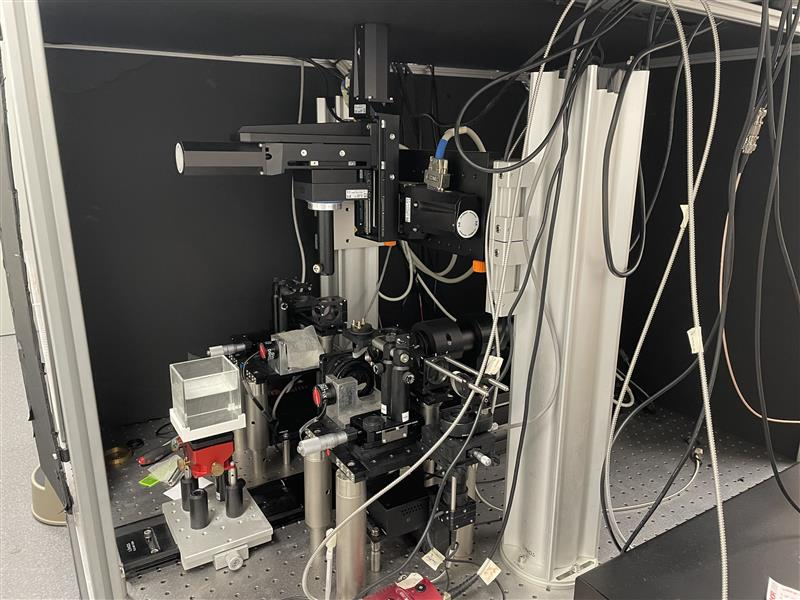
\includegraphics[width=1\linewidth]{Images/OverviewPhoto.jpg}
    \caption{Overview photo.}
    \end{subfigure}
    \medskip
   
    \begin{subfigure}[b]{0.75\textwidth}
    \centering
    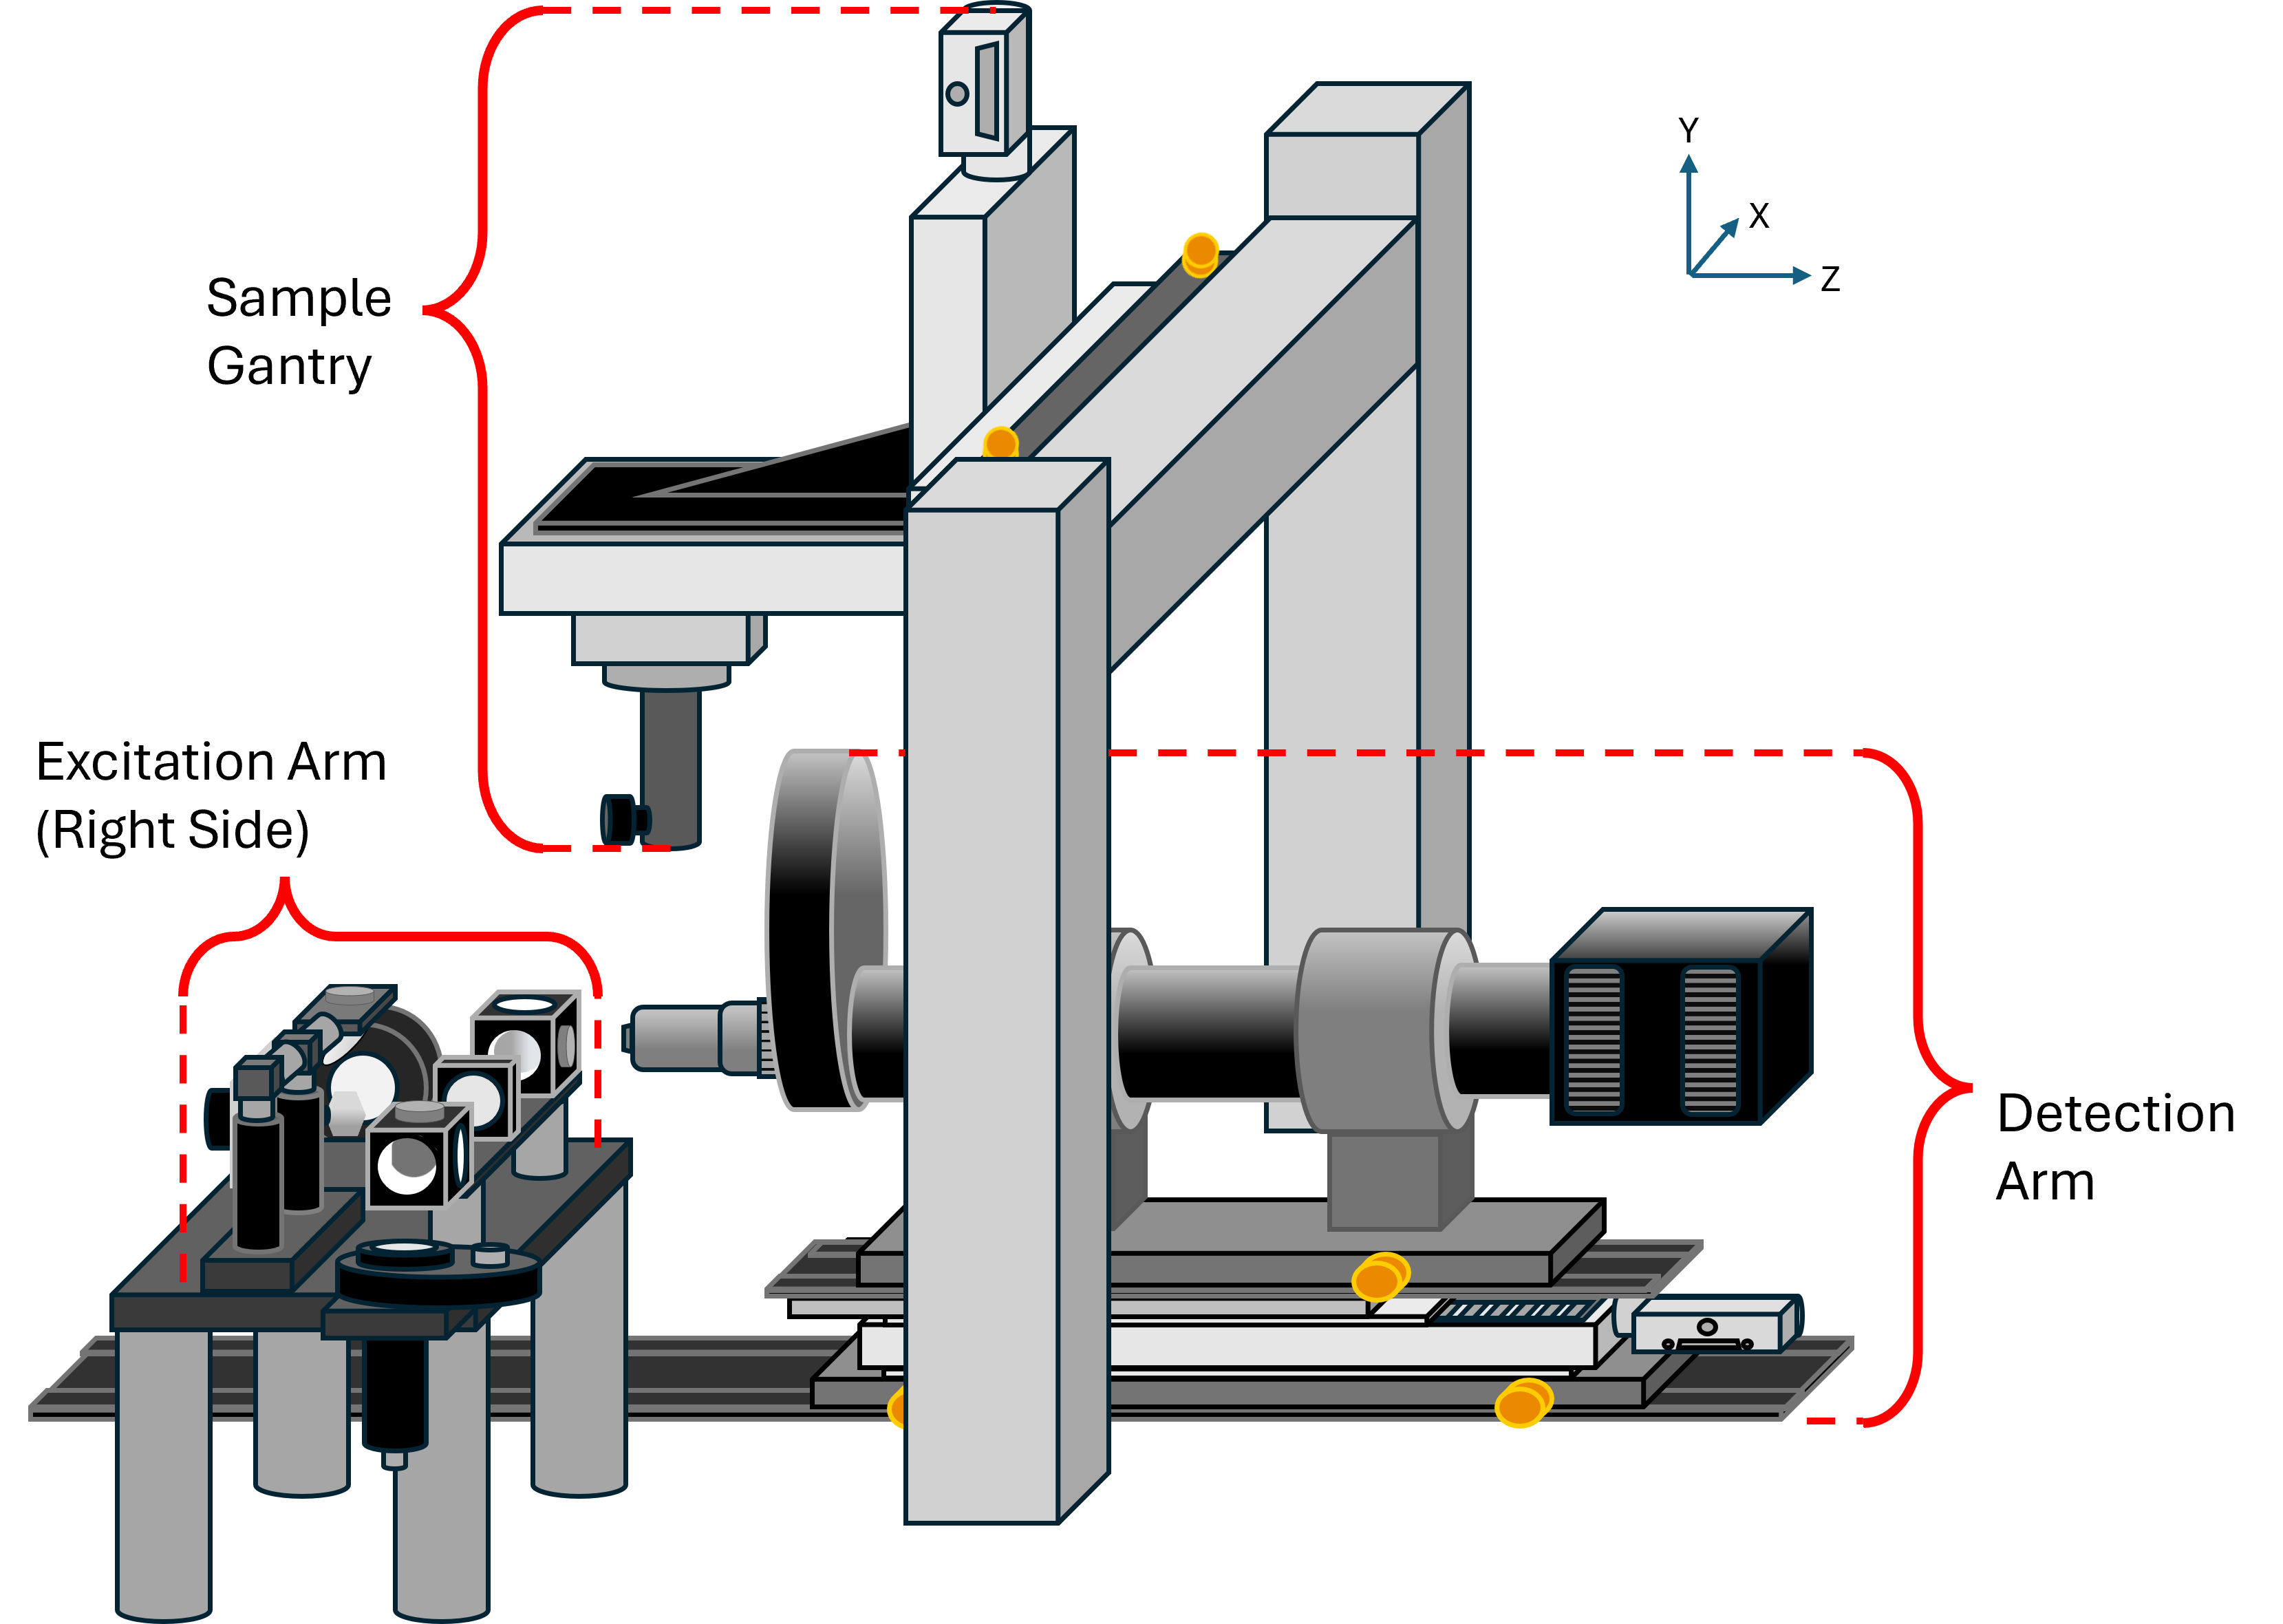
\includegraphics[width=1\linewidth]{Figures/Overview Diagram.png}
    \caption{Overview diagram. Isometric view from right side of system. Main components and location in overall setup highlighted. Additional structural supports, left side excitation arm, power/signal electrical wiring, and external dark box are not included in diagram for ease of viewing. (Diagram Not To Scale)}
    \end{subfigure}
   
   
    \caption{\textbf{Overview photo (a) and diagram (b) of fully assembled, upgraded ver.5 mesoSPIM}}
\end{figure}

The mesoSPIM microscopy system consists of three main components connected to a central PC that operates and synchronizes movement to permit light sheet imaging across mesoscale volumes with homogeneous, isotropic resolution in the range of 8-12 microns in the axial and lateral directions (See chapter 1, section 2.1 for LSM conceptual details). These three components includes the detection pathway, the single side excitation pathways, and the sample gantry. Table 2.1 details the resolutions achieved using this system in axial and lateral resolution as reported by the original system developers along with those resolution limits recorded  using the two unique imaging modalities performed with the system used during the course of this project.


\begin{table}[H]
    
    \begin{tabular}{|c|c|c|c|}
        \hline
         \textbf{Modality} &\textbf{ Lateral (X)} & \textbf{Lateral (Y)} & \textbf{Axial (Z)}\\\hline
         
         mesoSPIM Initiative Protocol \cite{voigt_mesospim_2019} & $1.5 \mu m $ & $1.5 \mu m$  & $3.3 \mu m$ \\
         
         Mounted Sliced Tissue Protocol & $4.66\pm0.67\mu m$ & $3.86\pm0.49\mu m$ & $7.76\pm1.64\mu m$\\
        
         Mounted Left Ventricle Section Protocol & $4.19\pm0.64\mu m $& 3.85$\pm0.42\mu m$ & 4.61$\pm1.12\mu m$\\\hline
       
    \end{tabular}
    \medskip
    \caption{\textbf{Resolution limits of upgraded Version 5 mesoSPIM microscope assembly utilizing established and experimental imaging modalities.} Details regarding mounted sample imaging protocols provided in Chapter 2, Section 3. Acquisition of resolution limits detailed in chapter 4, section 2.}
\end{table}

 


\subsection{Single Sided Excitation Pathway}
The first component of the mesoSPIM system are the excitation pathways located on elevated platforms to the immediate left and right of the detection pathway’s objectives. These pathways connect to the laser engine to the shutters, electronically tuneable lenses, and galvanometer mirrors that generate the axially scanning light sheet utilized by the mesoSPIM for imaging large tissue volumes (See Chapter 1, Section 2.2 for ASLM conceptual details). An image and optical pathway diagram of the fully assembled and aligned right side excitation pathway is seen in Figure 2.2(a) and (b) below.

\begin{figure}[H]
    \centering
    \begin{subfigure}[a]{0.75\textwidth}
    \centering
    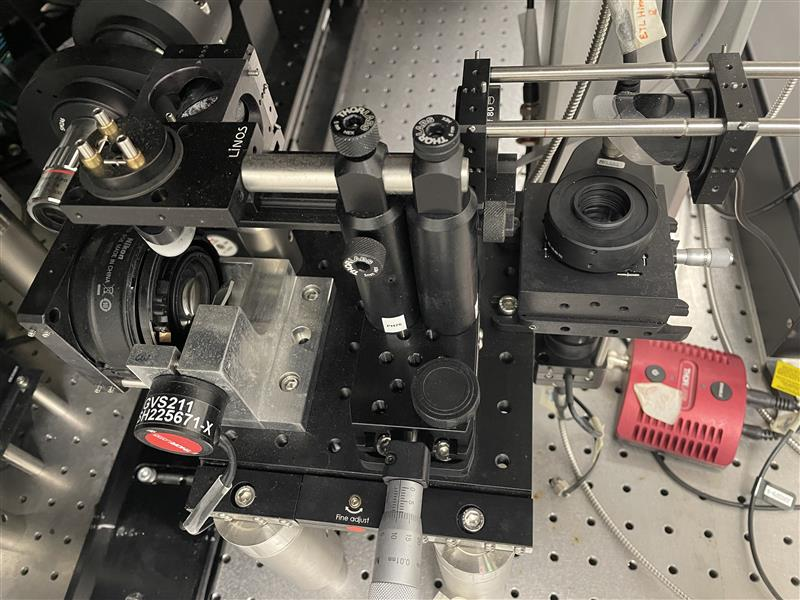
\includegraphics[width=1\linewidth]{Images/ExcitationPathPhoto.jpg}
    \caption{Photo of excitation pathway on right side of mesoSPIM.}
    \end{subfigure}
    \medskip
    
    \begin{subfigure}[b]{0.75\textwidth}
    \centering
    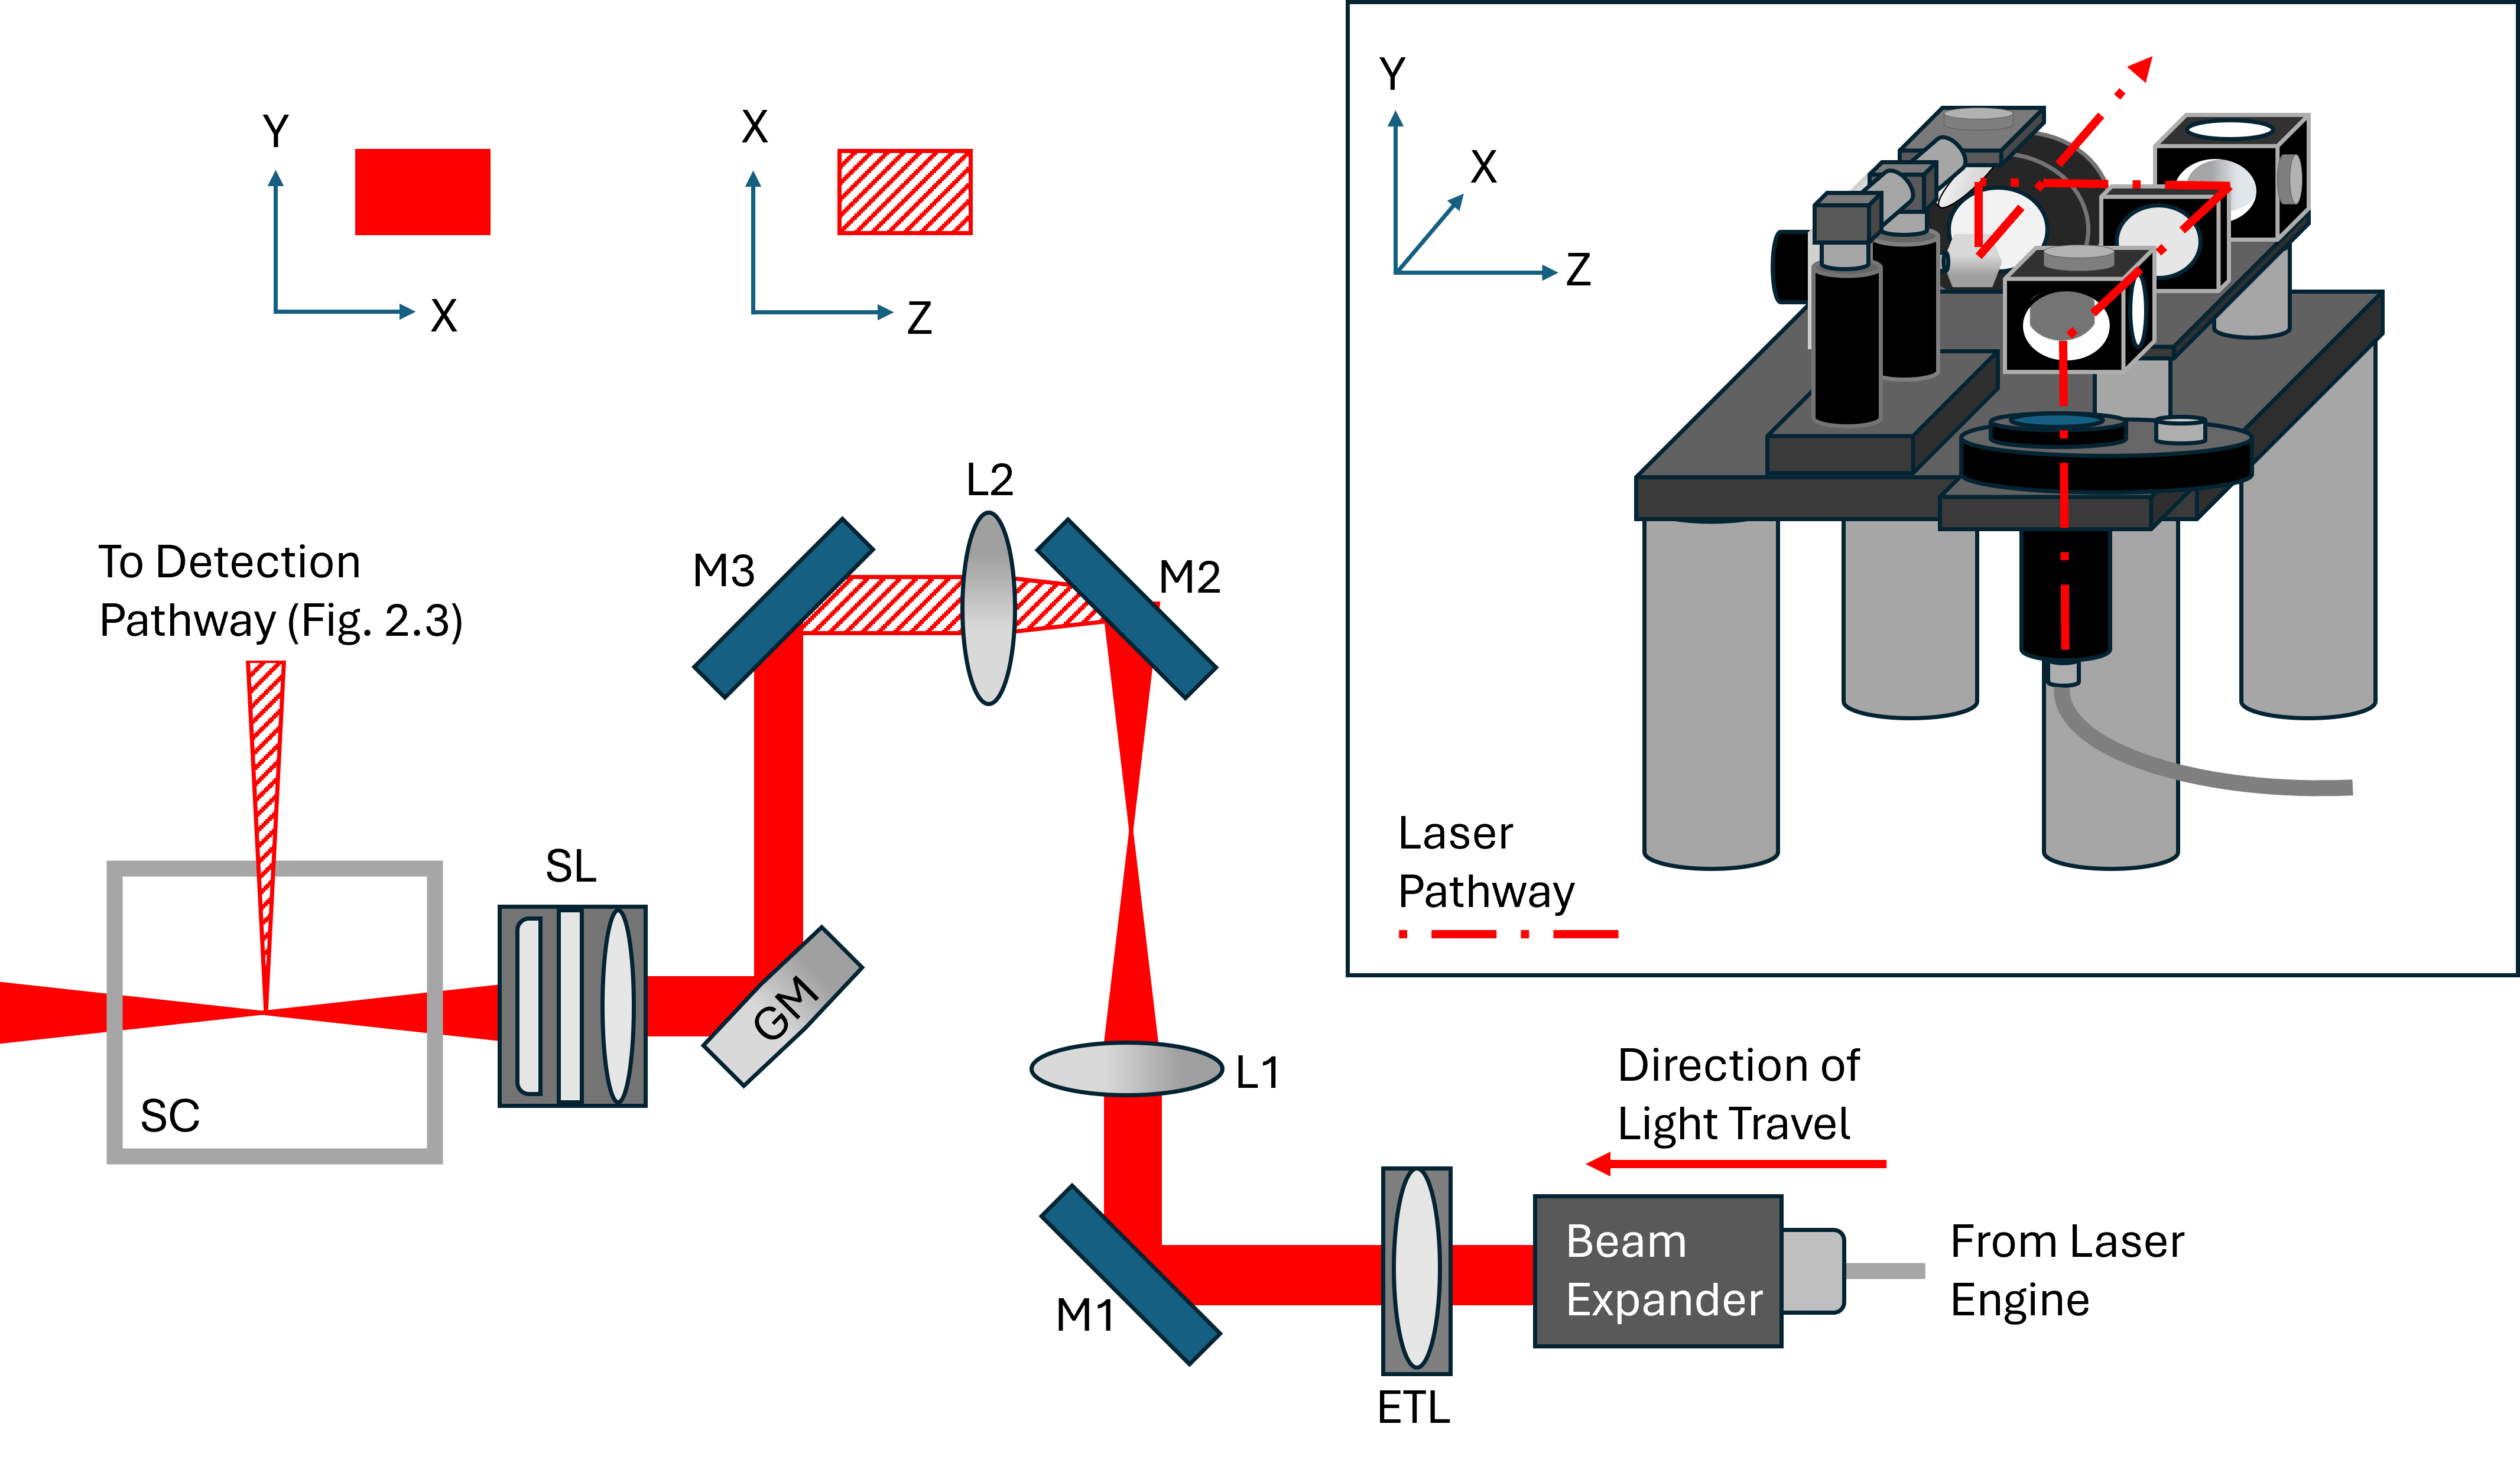
\includegraphics[width=1\linewidth]{Figures/Excitation Diagram.png}
    \caption{Excitation laser 2D and 3D (insert) optical pathway diagrams (Diagram not to scale). Legend - ETL: electronically tunable lens; M1-3: mirrors; L1-2: lenses; GM: galvonmeter mirror; SL: scan lens; SC: sample chamber. Left side excitation arm is YZ plane mirrored duplicate of right side arm.}
    \end{subfigure}
    \caption{\textbf{Fully assembled upgraded ver.5 mesoSPIM excitation pathway image (a) and diagrams (b)}}
    \label{fig:enter-label}
\end{figure}

A multiple channel laser engine (Omicron-Laserage GmbH, LightHUB ULTRA) was installed to generate the excitation beams used in the formation of the Gaussian beam. This engine allows for the installation of multiple laser lines with a custom selection of power levels and wavelengths which can be installed and uninstalled at anytime by me without the need to send the device back to the manufacturer. The laser lines can be  activated and deactivated seamlessly through the engines proprietary software as well as the mesoSPIM General User Interface (GUI). Table 2.2 lists the laser lines installed in the laser engine for the purposes of research conducted in this project. 


\begin{table} [H]
    \centering
    
    \begin{tabular}{|c|c|c|c|}
            \hline
            \textbf{Laser Line} & \textbf{Wavelength} & \textbf{Documented Max Power}\\ \hline
             
            LuxX CW Diode Laser 647& 647nm & 140mW\\
            
            OBIS LS Laser 532 & 532nm & 120mW\\
        
            LuxX CW Diode Laser 488 & 488nm & 100mW\\
           
            LuxX CW Diode Laser 405&  405nm & 120mW\\ \hline
    \end{tabular}
    \medskip
    \caption{\textbf{Laser lines installed into LightHUB Ultra\textsuperscript{\textregistered} Laser Engine}}
    \medskip
\end{table}

Following from the emission of the laser beam in the laser engine, the beam proceeds to pass through a beam expander followed by Electronically Tuneable Lenses (Optotune, EL-16-40-TC-VIS-5D-1-C) installed into each excitation arm. These ETLs allow the narrowest region of the Gaussian beam to shift (in x-axis) across the imaging field of view, as is required for axial scanning to occur. Continuing from the ETL aperture, the beam is reflected off of galvo scanning mirror (Thorlabs GVS211) directly into the back focal plane of modified Nikon camera lenses (AF-S 50mm f/1.4G). These lenses have had their internal apertures set to fully open, allowing them to acts as an f-theta configured objective lenses. The galvo scanning mirror allows the 10 mm diameter beam (Numerical Aperture, NA = 0.1) to shift back and forth in the y-axis to form the light sheet inside the sample chamber that can provide homogeneous illumination for sample imaging.

Assembly of the excitation arm structural supports, electrical wiring, and elevated platforms were completed by myself. Delicate modifications to Nikon scan lenses required for installation into the pathway were also completed carefully myself to avoid damage \cite{vladimirov_mesospimbenchtop-hardware_2025} This included the removal of sections of the external lens frame as well as the locking in place of the internal aperture of the lens to the fully open position. Caution was taken during these steps to not scratch or damage the lens as these alterations were made. Installation and Alignment of the optical components of the excitation arms were completed by Dr. Sharika Mohanan in accordance with alignment protocols provided by the mesoSPIM Initiative \cite{vladimirov_mesospimbenchtop-hardware_2025}. 

For the purposes of our research, all imaging was completed using only the excitation pathway on the right side of the detection pathway. This was done to allow full laser engine power (100 mW to 140 mW) to be dedicated to a single excitation path instead of utilizing a beam splitter to split the emitted laser across both pathways, cutting the maximum excitation laser power achievable by the system in half in the process (50 mW to 70 mW). Though inactive, the right side excitation arm was kept intact for use in imaging should the left side arm at any point encounter technical or optical issues. Beam splitter, fibre switch, and other components required to permit dual side illumination were also kept installed into the system or stored nearby for potential future use should higher power laser lines be installed into the laser engine.

\newpage

\subsection{Detection Pathway}
The detection pathway consists of (following the direction of emitted light travel): the microscope objective, emission filter wheel, tube lens, and finally an sCMOS camera. An image and diagram of the fully assembled detection pathway are shown in Figure 2.3(a) and (b) respectively.

\begin{figure}[H]
    \centering
    \begin{subfigure}[a]{1\textwidth}
    \centering
    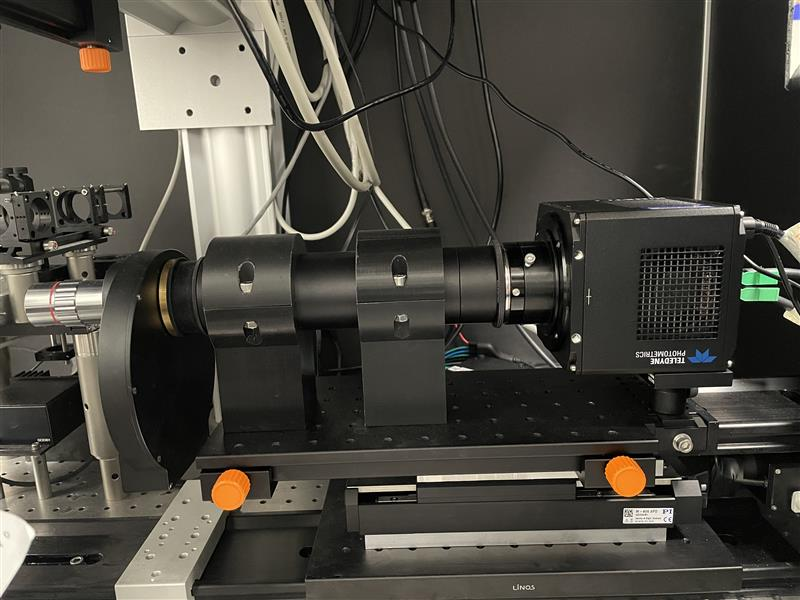
\includegraphics[width=0.75\linewidth]{Images/DetectionPathPhoto.jpg}
    \caption{Photo}
    \end{subfigure}
    \medskip
   
    \begin{subfigure}[b]{1\textwidth}
    \centering
    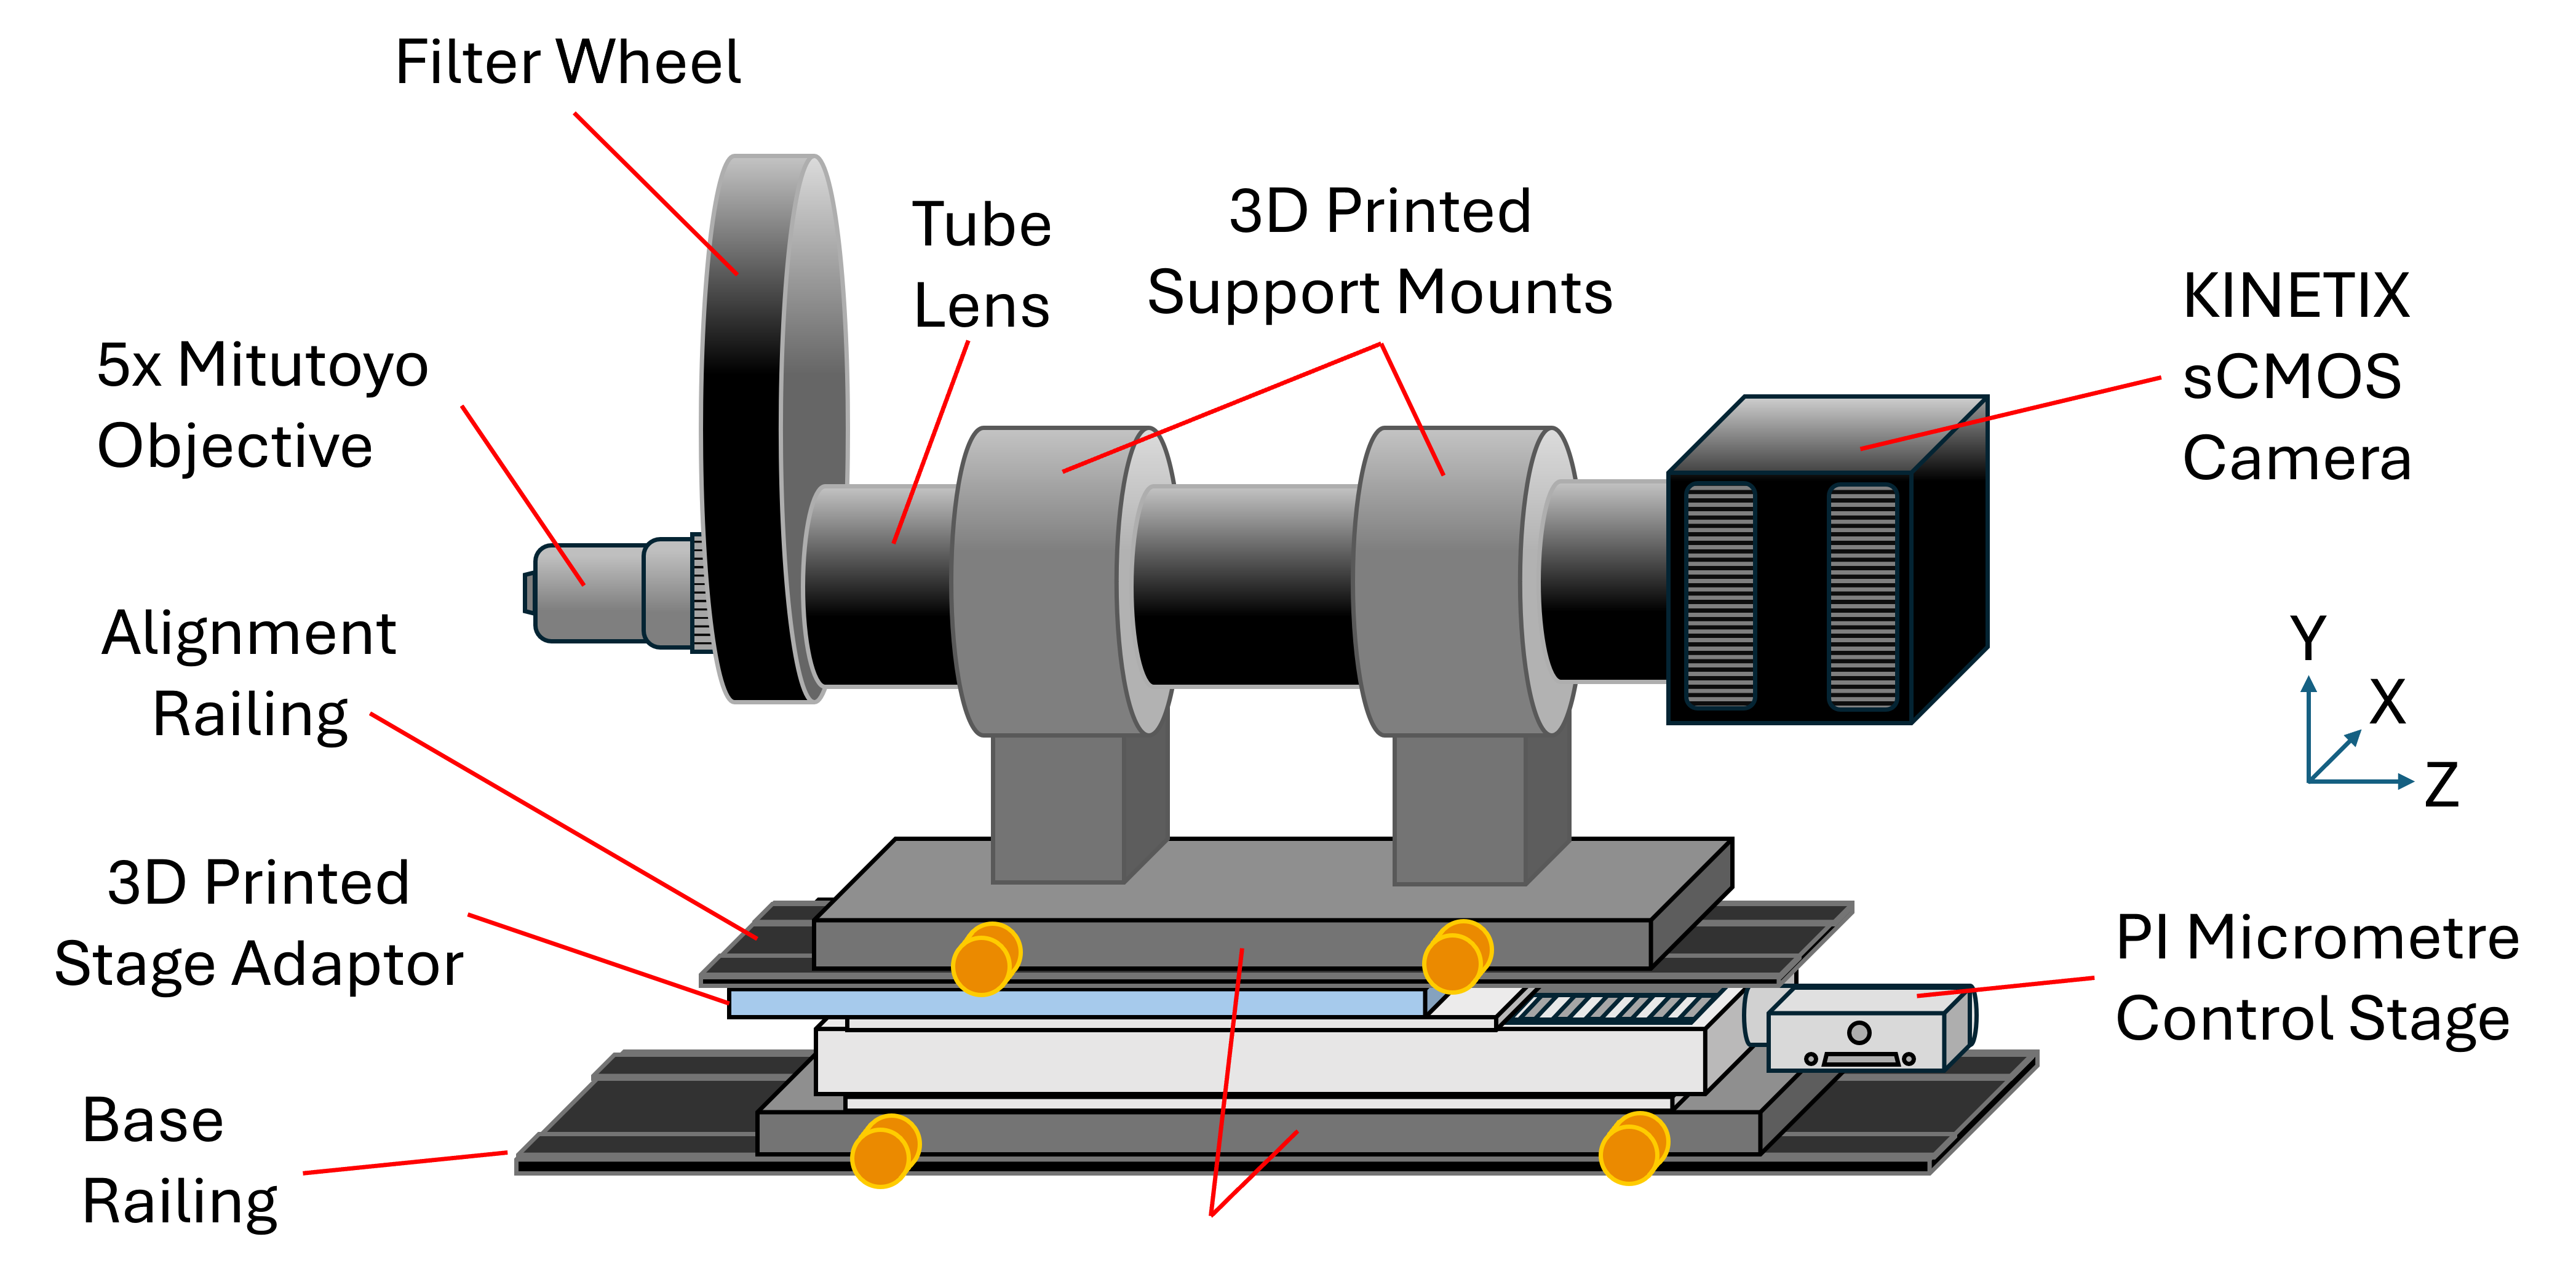
\includegraphics[width=1\linewidth]{Figures/Detection Diagram.png}
    \caption{Diagram}
    \end{subfigure}
    \caption{\textbf{Fully assembled upgraded ver.5 mesoSPIM detection pathway image (a) and diagrams (b)}}
    
\end{figure}


All 4 of these major components of the detection pathway sit atop motorized stage (Physike Instrumente, M-406.4PD) connected to a base rail spanning the length of the mesoSPIM assembly. This railing and stage assembly permits both manually coarse and electronically precise movement of the entire detection pathways for use in set up alignment and subsequent objective focus adjustment. The design is based on a upgraded version of the mesoSPIM version 5 detection pathway utilizing design features and 3D printed components created by the mesoSPIM Initiative for use in their most recent iteration of the system, the Benchtop mesoSPIM [23].

For this research, a single 5x Magnification Objective (Mitutoyo 5X EO M Plan Apo, 59-876, \textit{f} (focal length) = 50 mm, NA = 0.14) with a 34.0 mm working distance is utilized and connected directly to the front of the filter wheel via a lens tube adapter (Thorlabs SM2A6), allowing the lens to be removed and reattached without losing pathway alignment. Due to persistent technical issues, a Mitutoyo objective turret included in the original Benchtop mesoSPIM design was not implemented into the final version of the microscope's detection pathway used in image acquisition.

To simplify the changing of filters in the detection path, a 6 position, 25mm motorized filter wheel Filter Wheel For 36 mm Unmounted Filters (ZWO Electronics ZWO Z607-EFW-7X36- MKII) was installed into the detection pathway behind the objective lens. This filter wheel. This filter wheel allows for the emission filters, used to isolate light emitted from tissues from the fluorescent dyes, to be changed seamlessly through the mesoSPIM software without the need to disassemble the pathway to switch out filters between imaging sessions. A table of the filters available for use in the filter wheel during this research, and the associated laser wavelength range of transmission, is shown n Table 2.3: 

\begin{table} [H]
    \centering
    \begin{tabular}{|c|c|c|c|}
            \hline
            \textbf{Filter Name} & \textbf{Manufacturer}& \textbf{Filter Bandwidth}  \\ \hline
            
            445/45 BrightLine Basic\textsuperscript{\texttrademark}\ Single-Band Bandpass& Semrock & 422-467nm \\
            575/59 BrightLine\textsuperscript{\textregistered}\ Single-Band Bandpass & Semrock & 546-604nm \\
            514/30 BrightLine\textsuperscript{\textregistered}\ Single-Band Bandpass & Semrock & 500-529nm \\
            ET 655 Longpass Emission Filter & Chroma Technology & >655nm\\
             620/14 BrightLine\textsuperscript{\textregistered}\ Single-Band Bandpass & Semrock &  613-627nm \\ \hline
            
    \end{tabular}
    \medskip
    \caption{\textbf{Filters installed into the 6 positions of the ZWO electronic filter wheel}}
    
\end{table}

To capture the emitted fluorescent light as still images, a KINETIX sCMOS (scientific Complementary Metal–Oxide–Semiconductor) camera (Teledeyne Photometrics, 01-KINETIX-M-C) is attached to the end of the detection pathway. This sCMOS camera posses a 20.8 mm x 20.8 mm field of view with a pixel size of 6.5 mm x 6.5 mm. The KINETIX camera is capable of detecting light emitted at wavelengths from 200 nm to 1000 nm. Settings and parameters assigned to the mesoSPIM system detection pathway and KINETIX camera are provided in the python scripts in the GITHUB repository made for this project (URL HERE).



\subsection{Sample Gantry}
The third component of the mesoSPIM system is the sample gantry, which I mounted onto a steel archway constructed directly above the detection pathway and just behind the elevated platforms of the dual excitation pathways. An image and diagram of the fully assembled sample gantry can be seen in the Figure 2.4(a-b).

\begin{figure}[H]
    \centering
    \begin{subfigure}[a]{1\textwidth}
    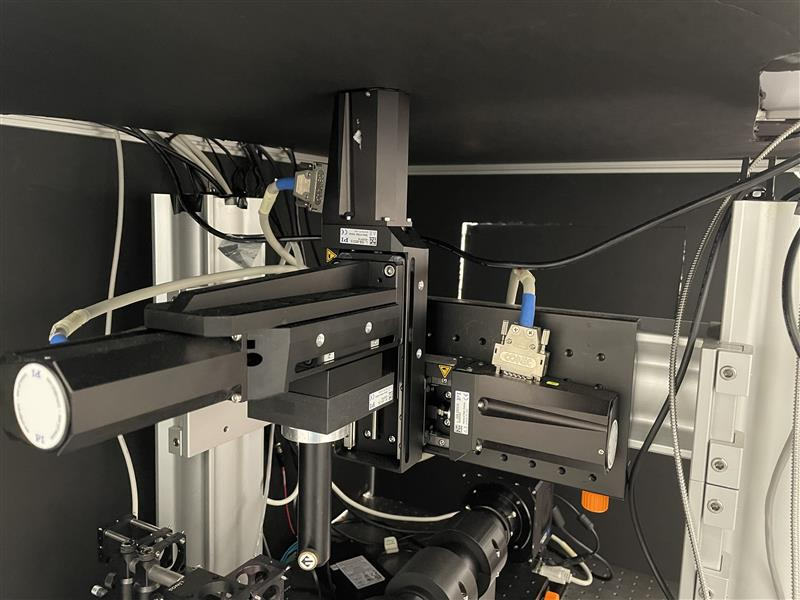
\includegraphics[width=0.875\linewidth]{Images/GantryPhoto.jpg}
    \caption{Photo of sample gantry}
    \end{subfigure}
    \medskip
    \begin{subfigure}[b]{1\textwidth}
    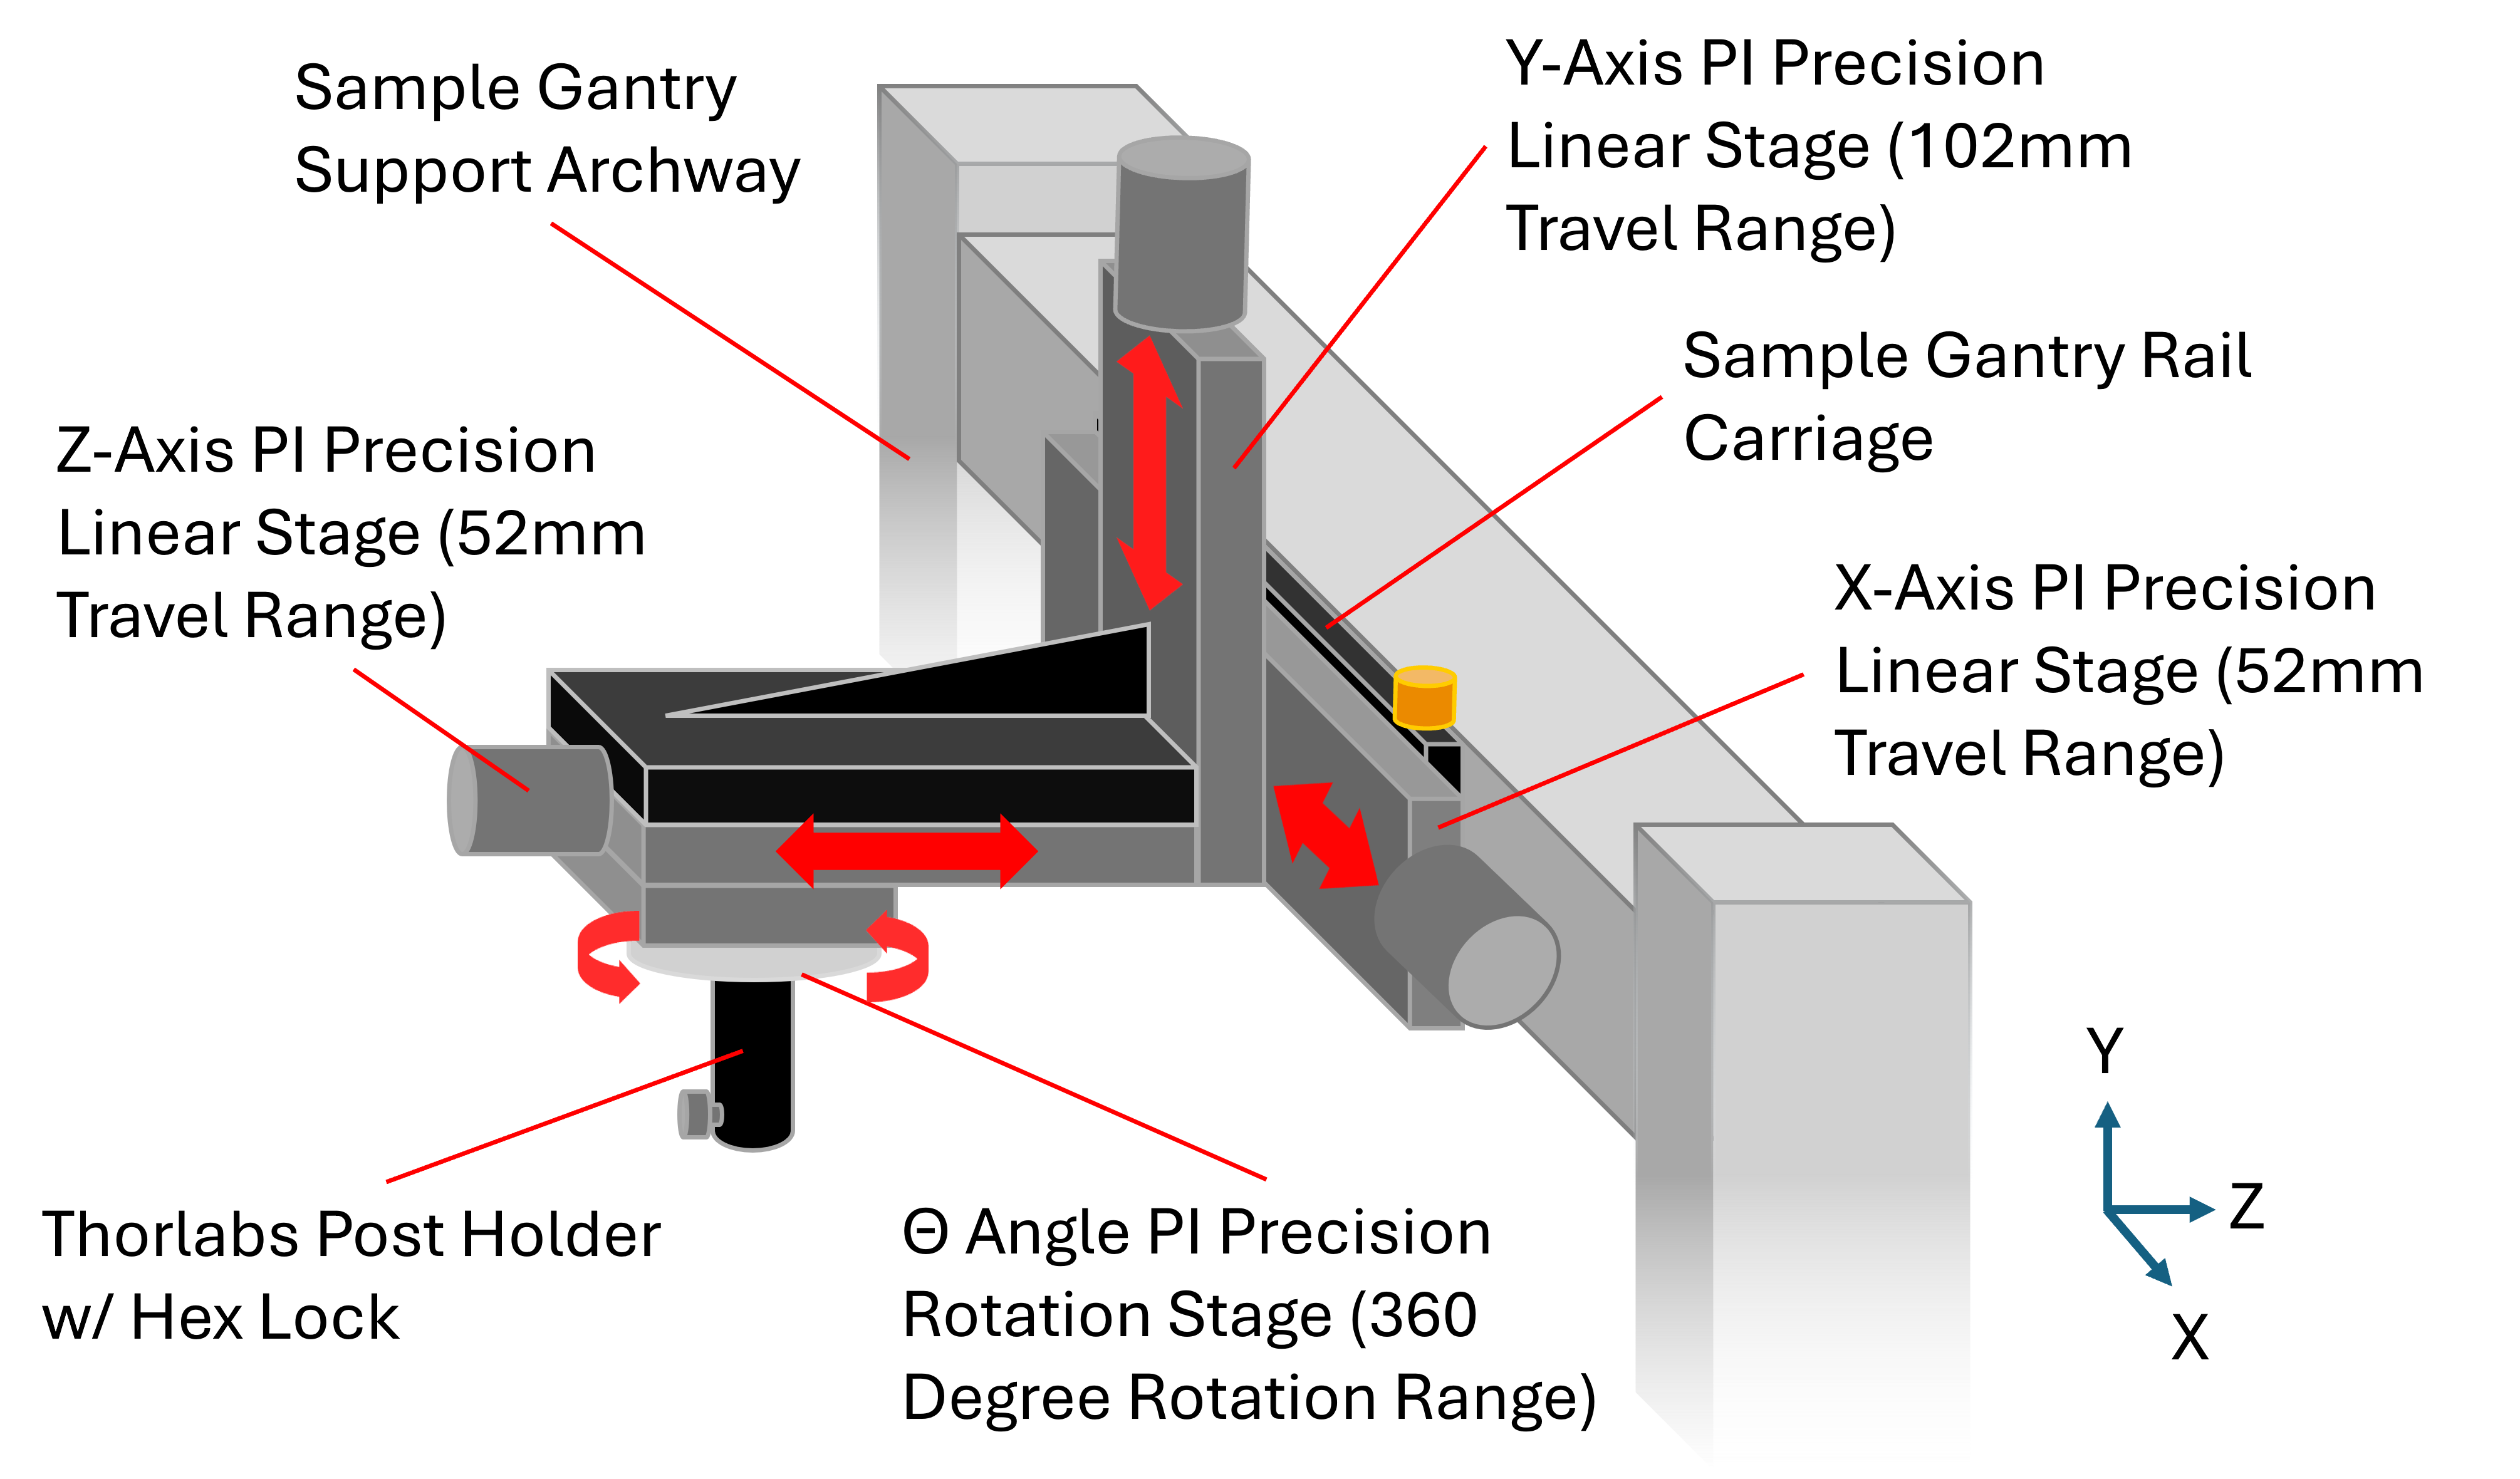
\includegraphics[width=0.875\linewidth]{Figures/Gantry Diagram.png}
    \caption{\textbf{Diagram of sample gantry components.} Stage axes of movements highlighted with red arrows.}
    \end{subfigure}
   
   
    \caption{\textbf{Fully assembled upgraded ver.5 mesoSPIM sample gantry photo (a) and diagram (b)}}
\end{figure}

This component of the system consists of 4 motorized stages (Physike Instrumente; PI L-509.40DG10, PI M-060.DG, PI L-509.20DG10(x2)) suspended directly above the intersection of the detection and excitation optical pathways. These stages are connected by a rail carriage attached and secured tightly to the side of the steel frame archway. The stages are connected one on top of the other to permit movement of the samples attached to the gantry in the x, y, z axes in addition to allowing full 360-degree rotation in the y-axis. 


\section{Data Acquisition}
\subsection{mesoSPIM Mounting}

To capture images of samples that need to be mounted into the mesoSPIM, the following series of protocols are implemented after completing the start up sequence of the mesoSPIM hardware and software. 

\subsubsection{\textit{External Immersion Imaging Cuvette Mounting Protocol}}
With the mesoSPIM software is fully activated and ready to start imaging of tissue samples, the tip-tilt plate platform is unlocked from the detection path railing and moved manually away from the objectives and camera in my direction. Once the tip-tilt plate atop the external cuvette platform is the furthest distance away from the objectives and the illumination pathway platforms, a custom ordered large volume cuvette (Portmann Instruments UQ-753) is then attached to the tip-tilt plate’s lower half magnetic connector (Thorlabs KBB1X1) using a custom designed, PLA 3D printed cuvette base mount. An image of this mount attached to the tip-tilt plate along with schematic detailing the dimensions of this custom designed mount is seen in Figure 2.7(A)and (B). Details on fabrication and design can be found in Appendix A. 

\begin{figure}[H]
    \centering
    \begin{subfigure}[a]{1\textwidth}
    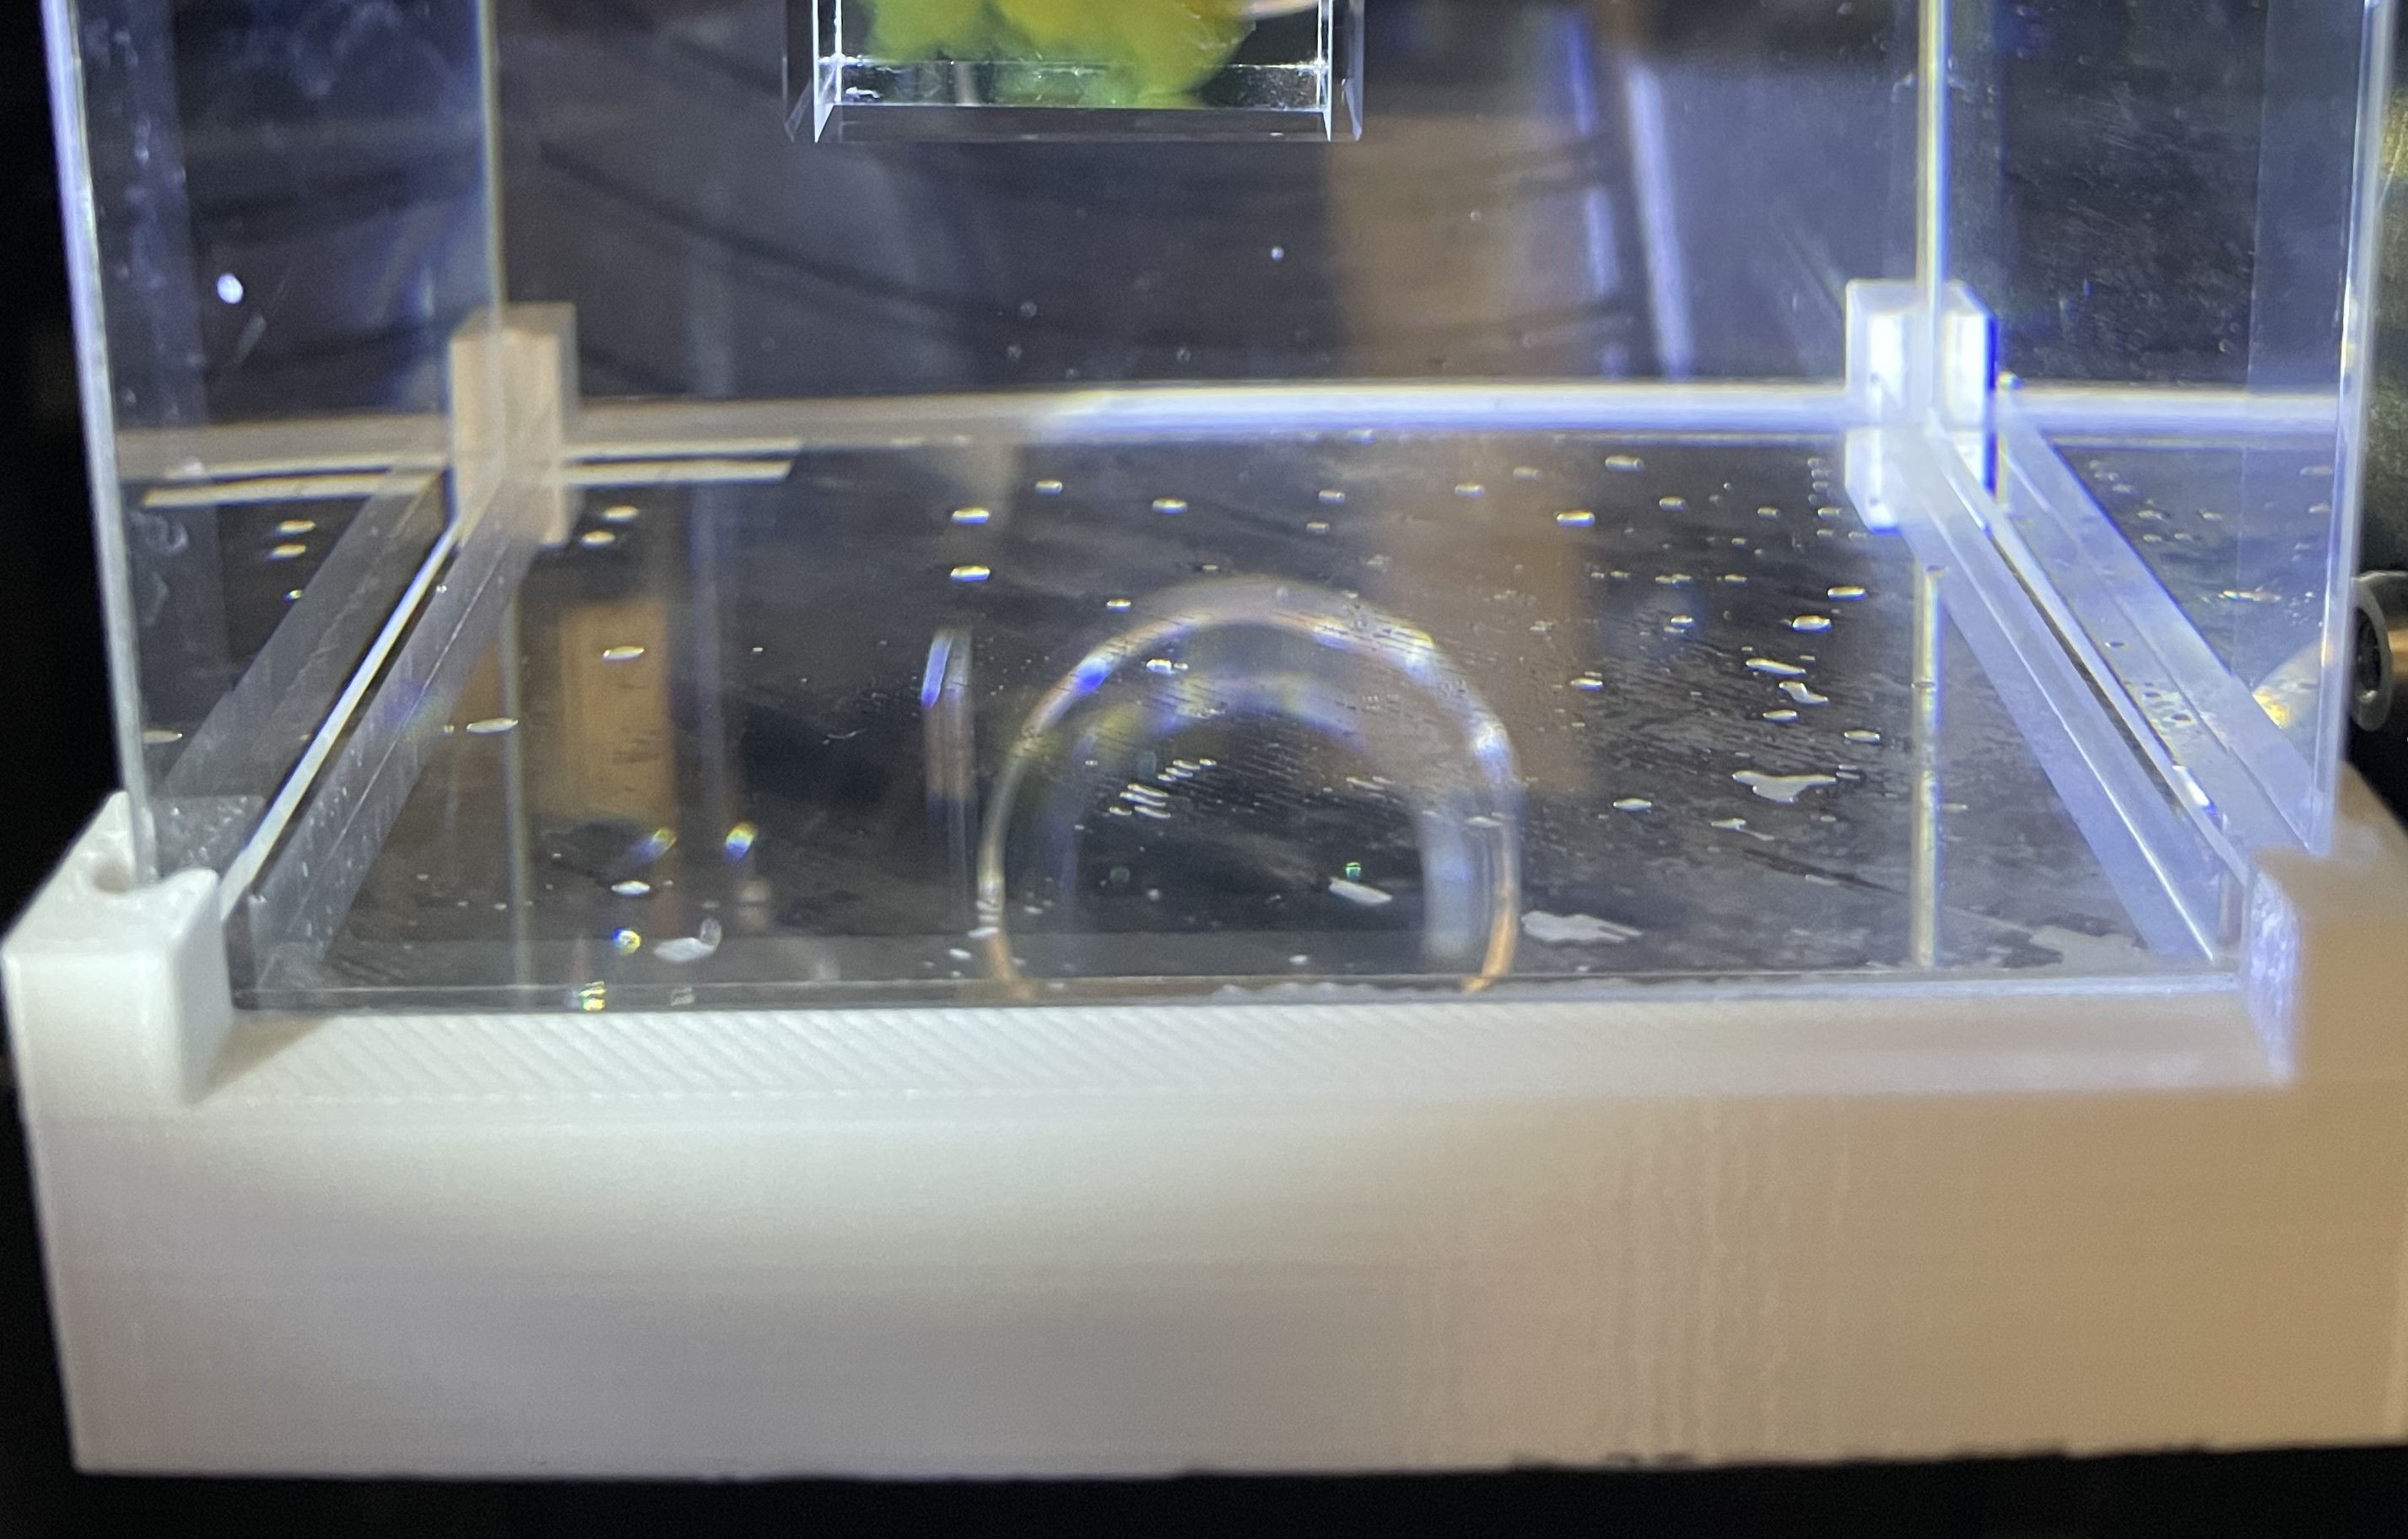
\includegraphics[width=1\linewidth]{Figures/ExternalCuvetteMount.jpg}
    \caption{Photo}
    
    \end{subfigure}
   
    \begin{subfigure}[b]{1\textwidth}
    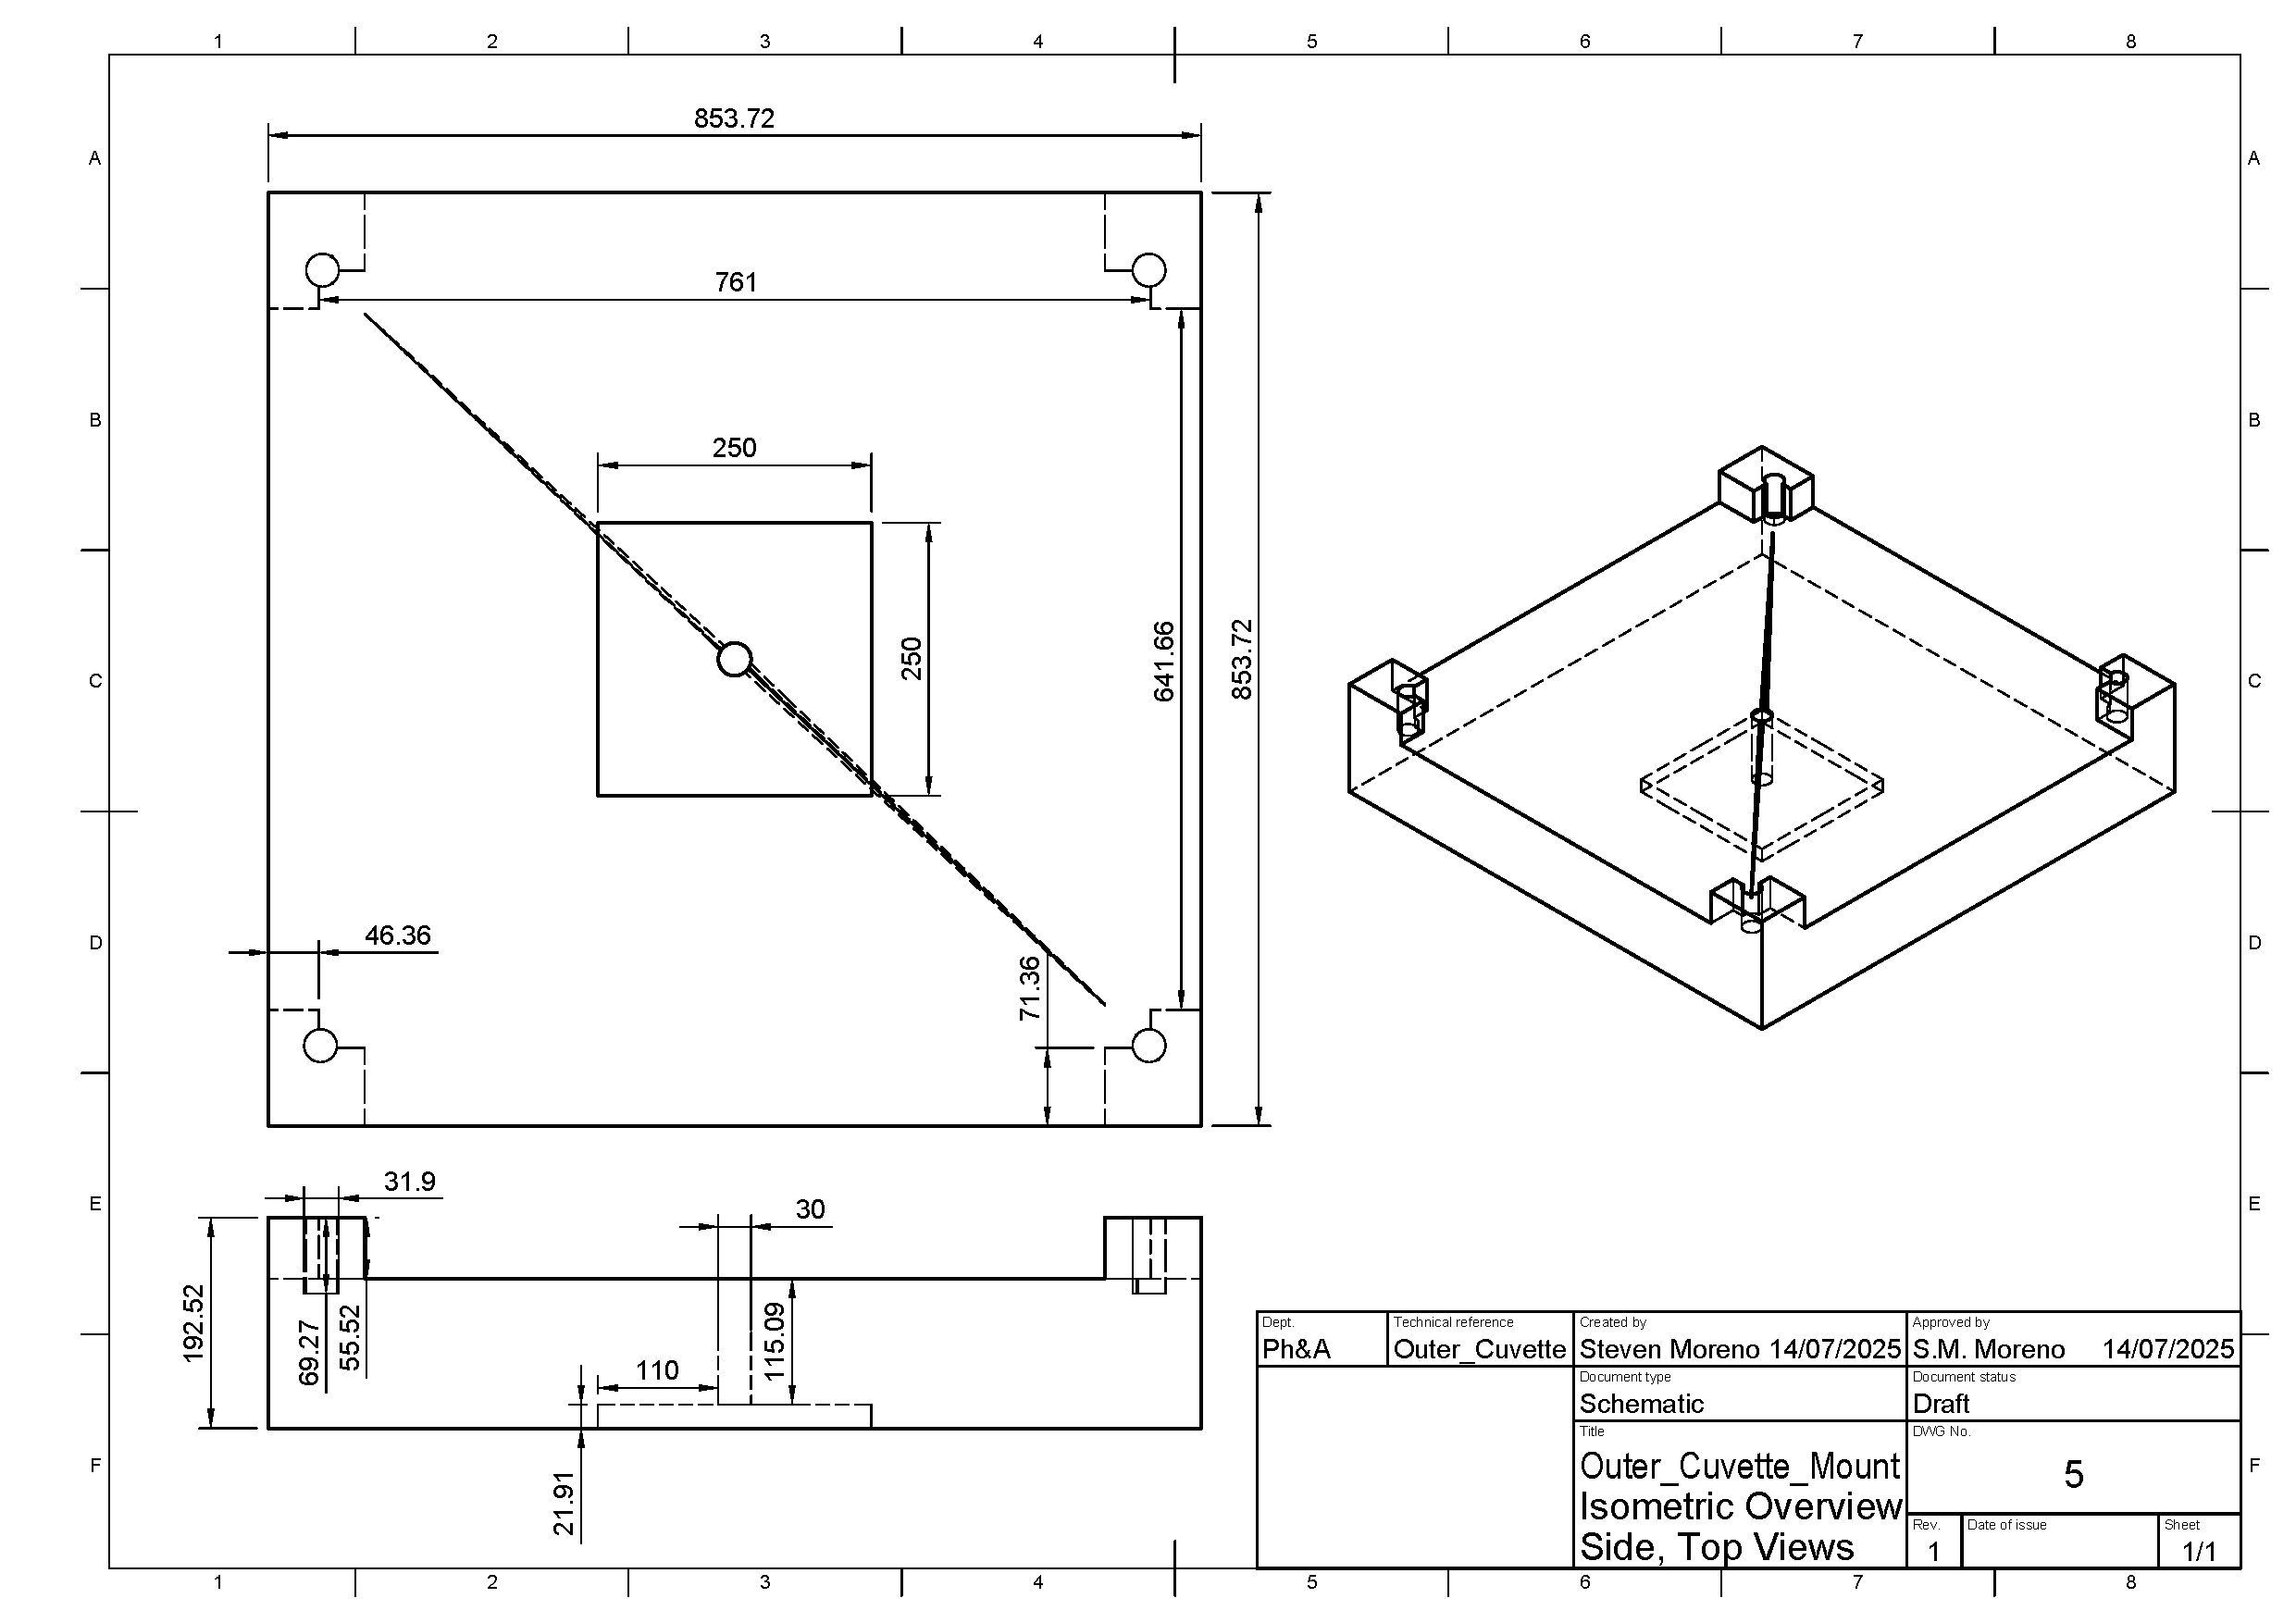
\includegraphics[width=1\linewidth]{Figures/Outer_Cuvette_Mount Drawing v1.pdf}
    \caption{Schematic}
    \end{subfigure}
    \caption{\textbf{Photo (a) and schematic (b) of custom PLA 3D-printed external cuvette mount.} Schematic created in Autodesk Fusion 360. Schematic side and front views to scale (1:5), orthogonal view not to scale}.
    \label{fig:enter-label}
\end{figure}

On the underside of the custom 3D printed mount is attached the upper half of the magnetic base connector (Thorlabs KBT1X10). With the external cuvette carefully inserted into the mount, the magnetic base on the top of the tip-tilt plate is connected to the magnetic base on the bottom of the custom mount. This process is done slowly by me to ensure any sudden jerk made by the magnetic connection does not cause any solution from spilling out of the external cuvette attached to the mount. Once the connection is made and the solution inside the cuvette has settled in movement, the cuvette platform is slowly returned to its original position on the detection pathway railing and locked backed into in place by tightening the hex screw on the side of the rail mount beneath the platform. 

\subsubsection{\textit{Sliced Tissue Sample Mounting Protocol}}
The sample gantry located directly above the external cuvette platform is then raised to the highest position in the y-axis using the mesoSPIM user interface. Tissue samples are placed into a custom designed spacer mount prior to attachment onto sample gantry (See chapter 4 for details). Mounted samples are then inserted into the inverted post holder (Thorlabs PH75/M) located at the bottom of the sample gantry. This post holder contains a 12.7 mm bore that fits the 3-D printed topper of the mounted tissue samples.  The sample is attached to the holder with the topper inserted fully into the holder ensuring the sample remains perfectly horizontal. The hex lock is then partially screwed in enough to hold the sample in place but still loose to allow mount to rotate freely inside the holder by rotating the mount manually by hand.

With the sample connected to the gantry, the mount is slowly lowered using the mesoSPIM GUI into the Refractive Index Matching Solution contained in the external cuvette located directly below the sample. Once the mount is approximately 3-4 mm from the base of the external cuvette, the gantry is moved in the z-axis to move the mount towards the wall of the external cuvette. I continue to move the sample until the mount is fully flushed against the wall of the cuvette. If the mount is not perfectly parallel to the wall of the cuvette, the mount is manually rotated inside the post holder until they have the mount become flush against the wall. Caution is used to ensure the mount does not push against the wall of the cuvette with excessive force to prevent scratching or cracks from forming. Once the mount is flushed against the wall, the hex lock on the side of the sample gantry post holder is fully locked in place. A photo showing the the mounted sample mid alignment, flushed against the wall of the external cuvette, can be seen in Figure 2.6.

\begin{figure}[H]
    \centering
    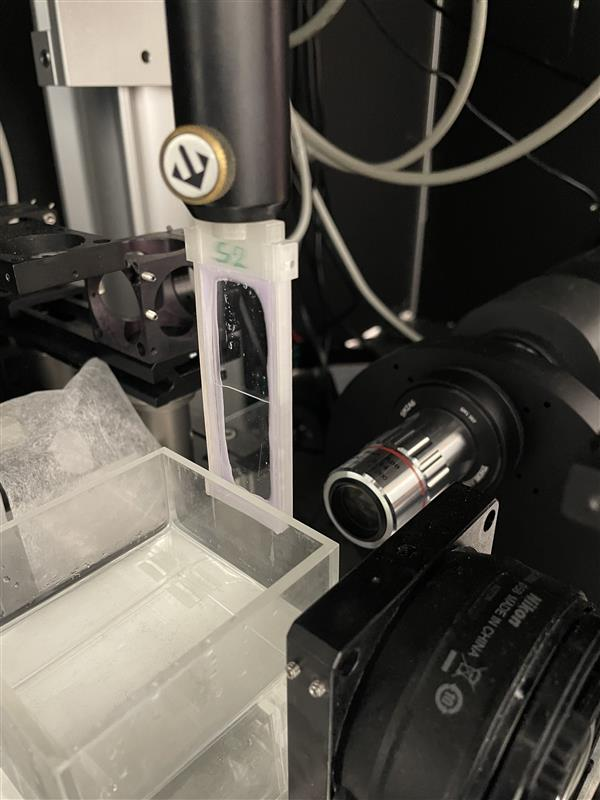
\includegraphics[width=0.5\linewidth]{Images/Alignment_Photo.jpg}
    \caption{\textbf{Photo of the alignment process of the sample mount with respect to the external cuvette walls.} }
    \label{fig:enter-label}
\end{figure}

The locked sample is raised by the sample gantry high enough to clear the top of the external cuvette, which is moved into position for imaging, indicated by a visible marking on the central optical rail indicating where the external cuvette platform should be positioned and locked into place to have the narrow waist region of the light sheet's Gaussian beam traverse through the midpoint of the cuvette's internal volume.


\subsubsection{\textit{Left Ventricle Tissue Mounting Protocol}}
Once the mesoSPIM is fully activated and ready to image samples, the tip-tilt plate platform is unlocked from the detection path railing and moved manually away from the objective and camera, in my direction.  With the tip-tilt plate atop the external cuvette platform a sufficient distance away from the detection arm components, the external soda lime glass external cuvette can then be safely attached to the tip-tilt plate’s lower half magnetic connector (Thorlabs KBB1X1) using the custom external cuvette base mount (see section 3.2). 

The sample gantry located directly above the external cuvette platform is then raised to the highest position in the y-axis using the mesoSPIM user interface. An inverted post (Thorlabs TR50/M) with a bottom half of a magnetic base connector attached at the bottom is then inserted fully into the sample gantry post holder (Thorlabs PH75/M). The hex screw on the side of the post holder is screwed tight to hold the post in place with the square magnetic mount sides oriented parallel to the detection and excitation pathways. A custom internal cuvette mount topper and suspension harness is attached to the upper half of the magnetic base connector (Thorlabs KBT1X1). The bottom half of the magnetic base connector is attached to a custom made, 3D printed cuvette holder (see Figure 2.7). This cuvette holder attaches to the open top of a soda-lime glass cuvette (Portmann Instruments UG-205, UQ-205) which itself is secured in place using 4 screws inserted to the sides of the mount that connects to a harness platform beneath the cuvette. 



\begin{figure}[H]
    \centering
    \begin{subfigure}[a]{0.25\textwidth}
    \centering
    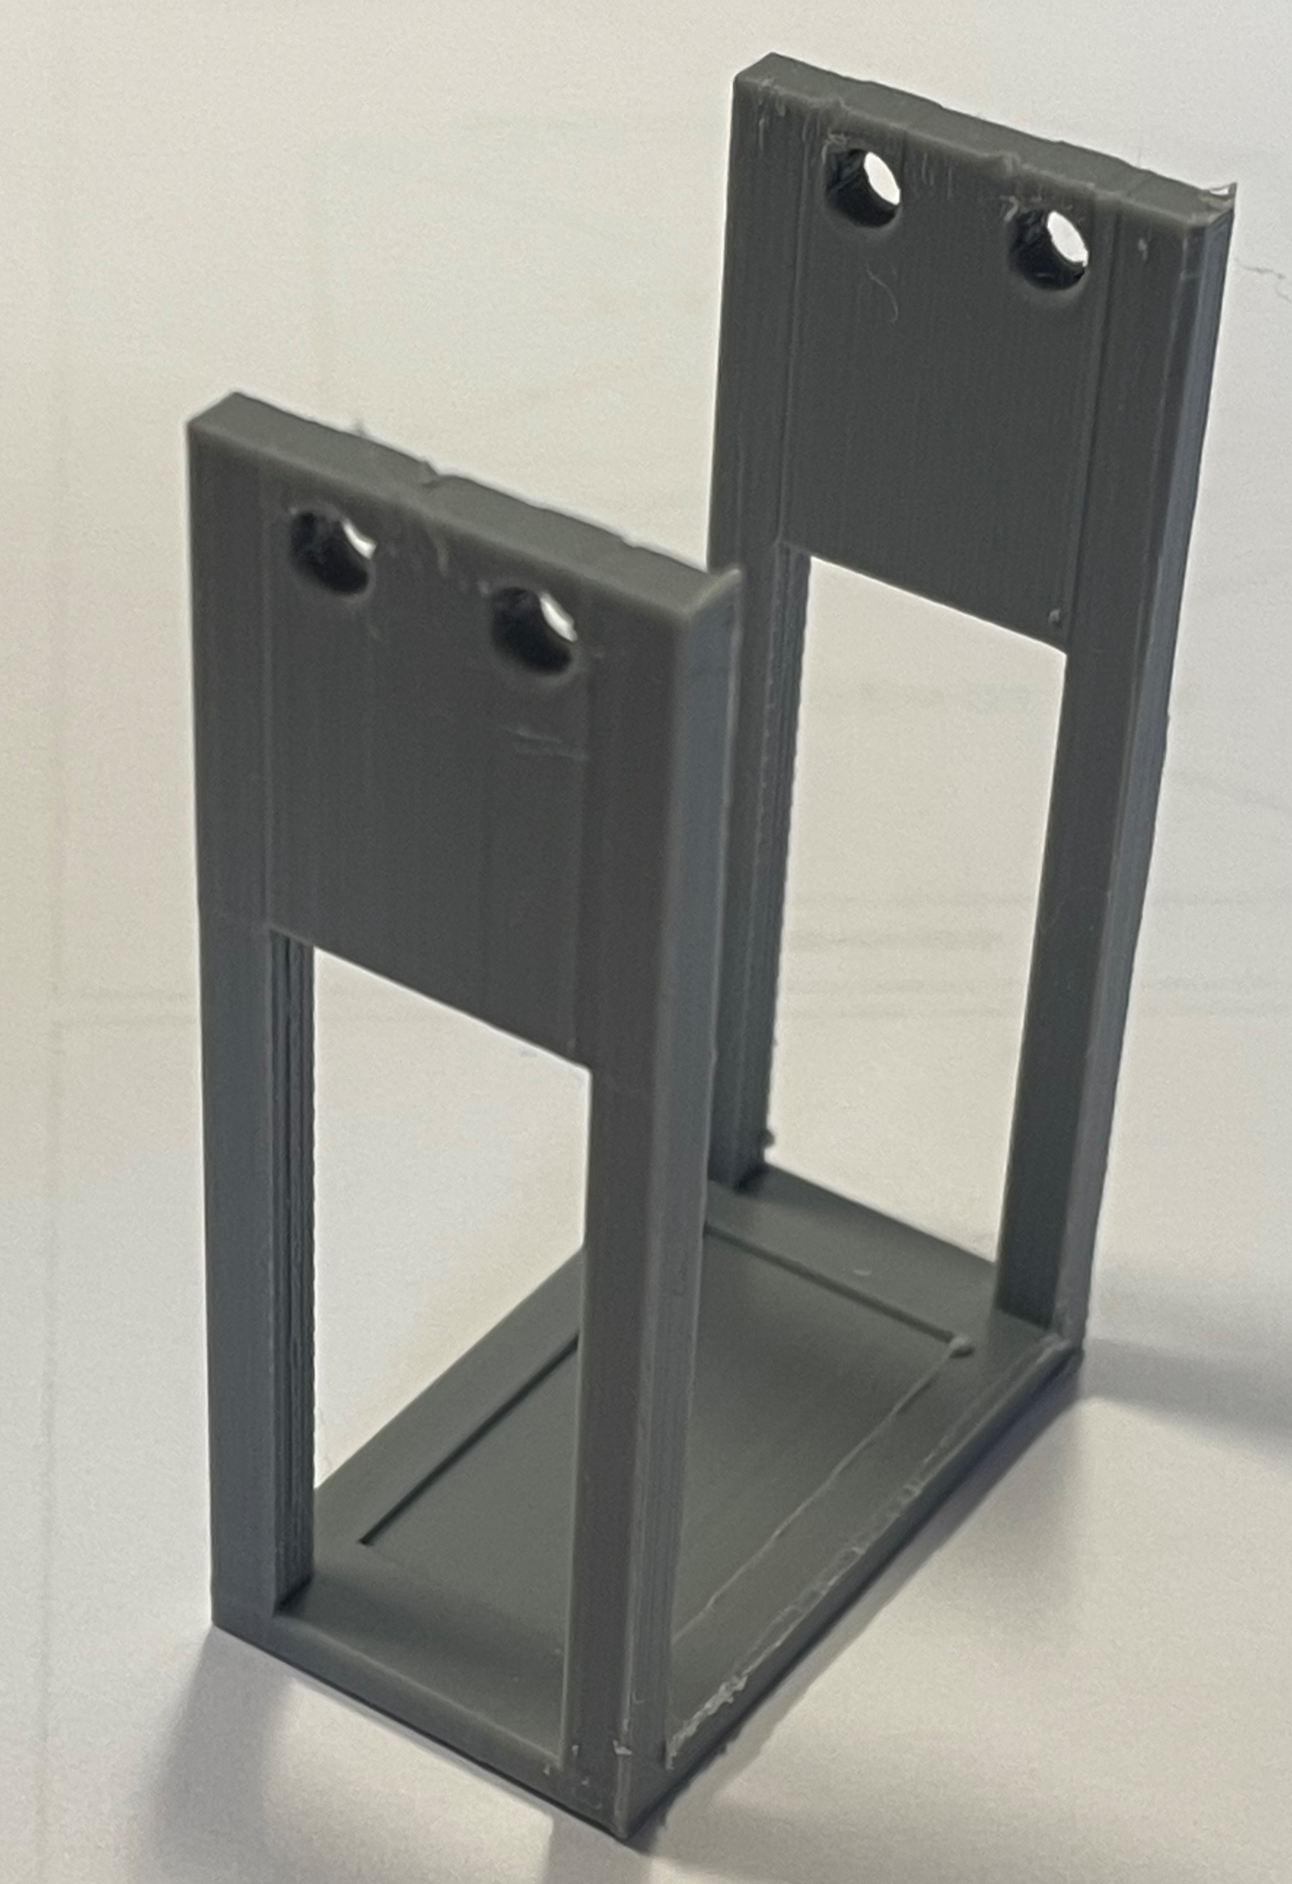
\includegraphics[width=1\linewidth]{Images/Lower_Mount.png}
    \caption{Inner cuvette mount base platform}
    \end{subfigure}
    ~ 
    \begin{subfigure}[a]{0.25\textwidth}
    \centering
    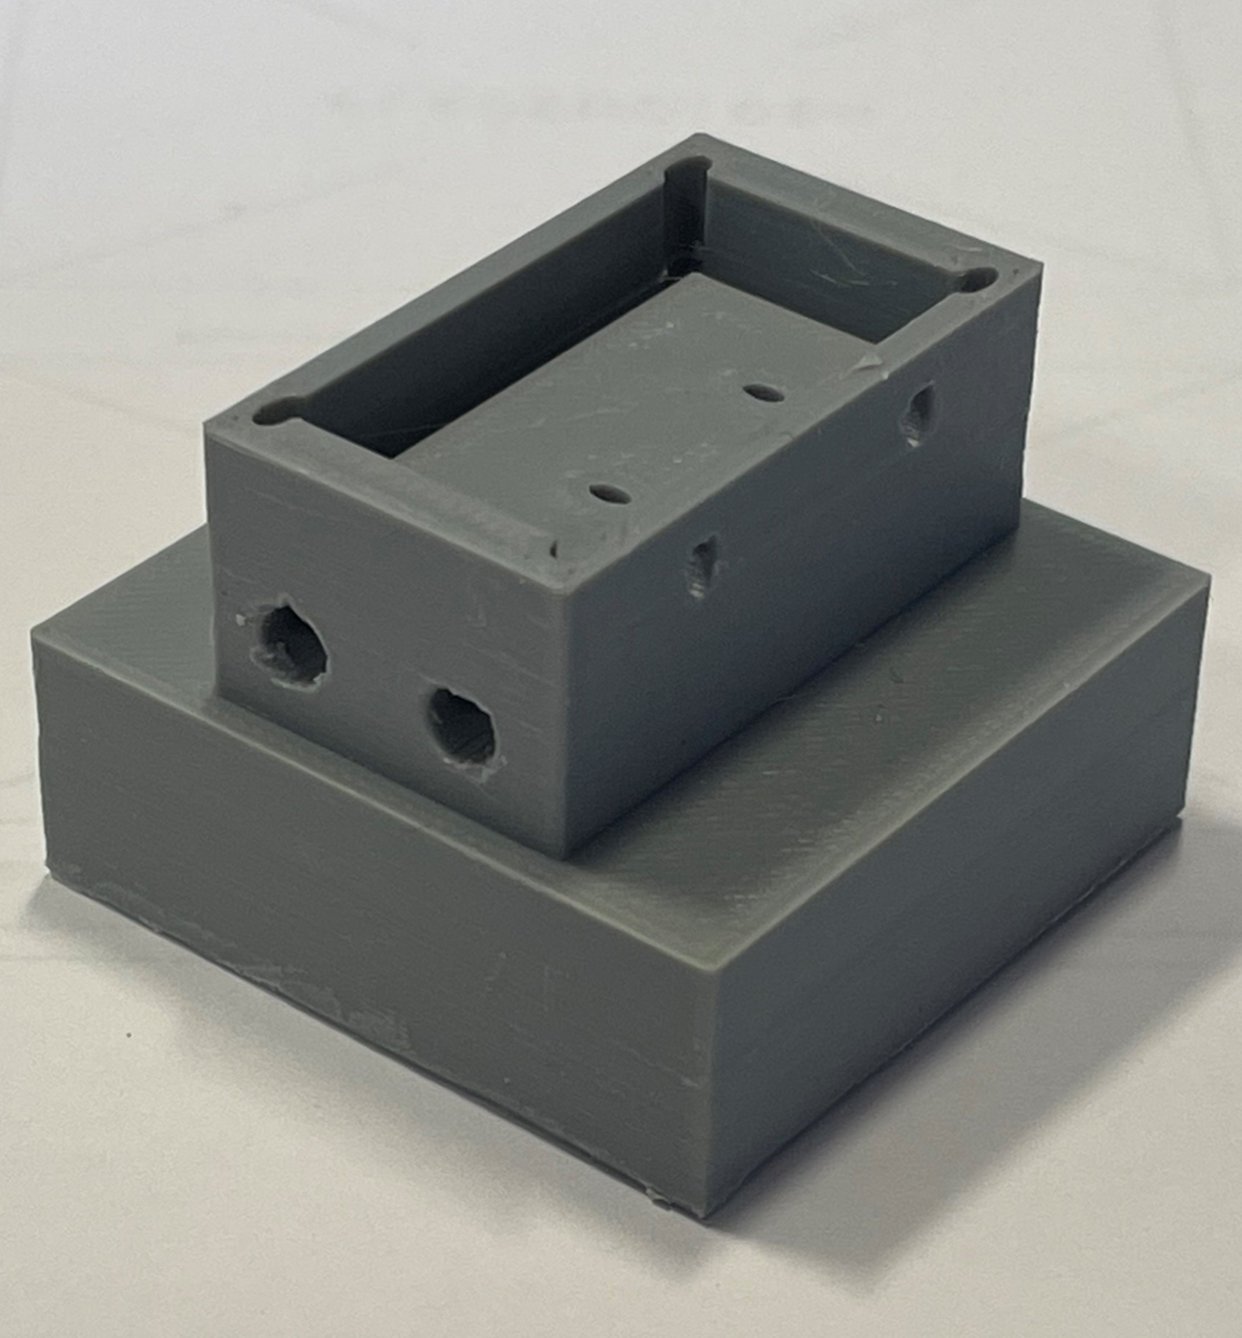
\includegraphics[width=1\linewidth]{Images/Upper_Mount.png}
    \caption{Inner cuvette mount topper}
    \end{subfigure}
    ~
    \begin{subfigure}[a]{0.25\textwidth}
    \centering
    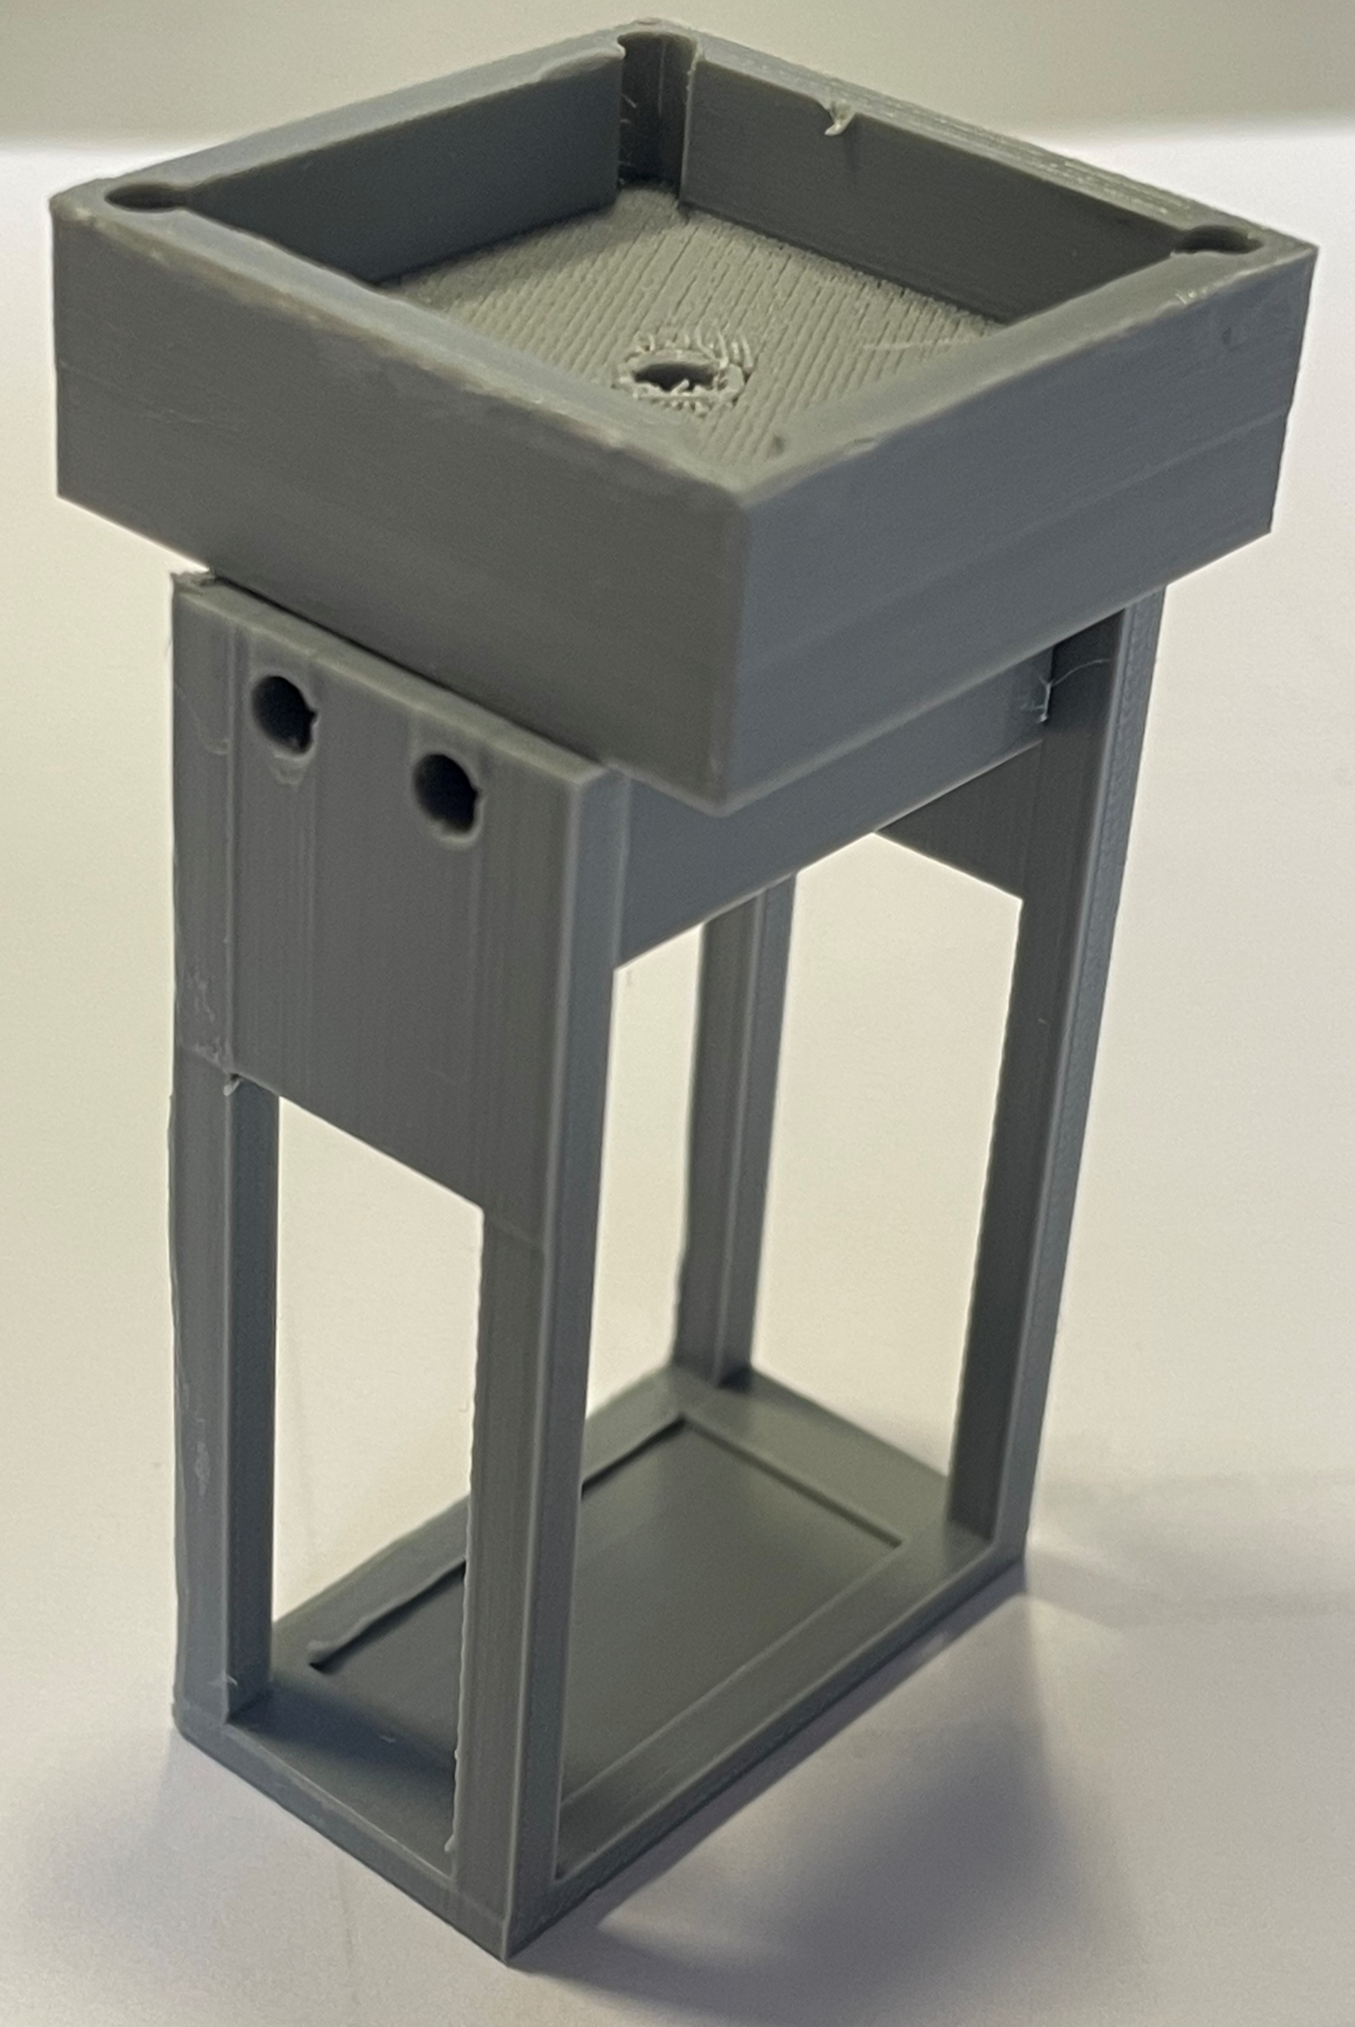
\includegraphics[width=1\linewidth]{Images/Combined_Mount.png}
    \caption{Assembled inner cuvette mount}
    \end{subfigure}
    
    \caption{\textbf{Photos of custom PLA 3D-printed internal cuvette mount.} Separate components shown in (a-b), components assembled together shown (c). Schematics Available in Appendix A. See Chapter 4 for design details.}
    
\end{figure}

The two halves of the magnetic base plate are connected, attaching the mounted cuvette to the bottom of the sample gantry. This process is done slowly by me to ensure the jerk of the magnetic connection does not cause any solution from spilling out of the external cuvette attached to the mount. Once the solution inside the cuvette has settled in movement, the external cuvette tip-tilt plate platform is returned to its original position on the detection pathway railing and locked in place. 

With the sample connected to the gantry, the mount is lowered into the Refractive Index Matching Solution contained in the external cuvette below the sample. The sample is lowered using the mesoSPIM GUI in increments of 0.5 mm to ensure the mounted internal cuvette does not collide with the base of the external cuvette. As the sample inside the inner cuvette reaches the same y-plane as the objective lens of the detection path, the mounted sample is then shifted in the z-axis until the inner cuvette is roughly on the z-axis of the excitation pathway scanning lens. I ensure the mount does not touch the walls of the outer cuvette at any point during positioning. 

\subsection{Imaging Protocols}

The foundations of tissue imaging methodologies discussed in this chapter were originally published by the mesoSPIM Initiative [2,23]. Changes made for operation of the mesoSPIM microscope for optimal performance as part of the overarching imaging pipeline will also be discussed here.

\subsubsection{\textit{Imaging Session Preparation}}
Once mounting protocols are completed and the mount is confirmed to be securely attached to the sample gantry, the 488nm laser line is set to 5\% power emission to allow for visual inspection of the light sheet formed inside the external imaging cuvette. The sample mount position is then carefully adjusted in the x,y, and z-axis until the tissue contained within the mount is in the pathway of the light sheet. The light sheet is confirmed to not be obstructed by any components of the mount to the left or right of the tissue (in the case of sliced tissues) or above/below the tissue (in the case of LV samples).

Once confirmed that the light sheet traverses across the tissue with no mount obstructions, the doors of the mesoSPIM dark box are closed, ensuring no light penetration in or out of system while the camera records and the laser lines operate at high power. The laser power emission is raised until a sufficient amount of illumination is obtained from the tissue (see parameter table in Appendix D for power levels used in data acquisition). The live camera image displayed on the PC by the mesoSPIM GUI software is  utilized to adjust the emission level, objective focus, and ETL settings of the mesoSPIM until a homogeneously bright, clear and focused image of the tissue is obtained. 

\subsubsection{\textit{ETL Parameter Selection}}
Using the mesoSPIM user interface, the electronically tuneable lenses are then adjusted by freezing the galvanometer mirror movement and zeroing the lens amplitude voltage, allowing the stationary Gaussian beam waist to be observed by the camera system. The beam waist is adjusted using ETL setting options in the software to have the narrowest region of the waist positioned at the centre of the camera field of view. The amplitude setting of the ETL is then adjusted to have the narrowest region of the Gaussian beam waist extended to cover as much of the field of view as possible. The Gaussian Beam should appear in the end of this process as a straight, narrow beam line across the field of view, seen as both a recorded image and a reference diagram in Figure 2.8.

\begin{figure}[H]
    \centering
    \begin{subfigure}[t]{0.4\textwidth}
    \centering
    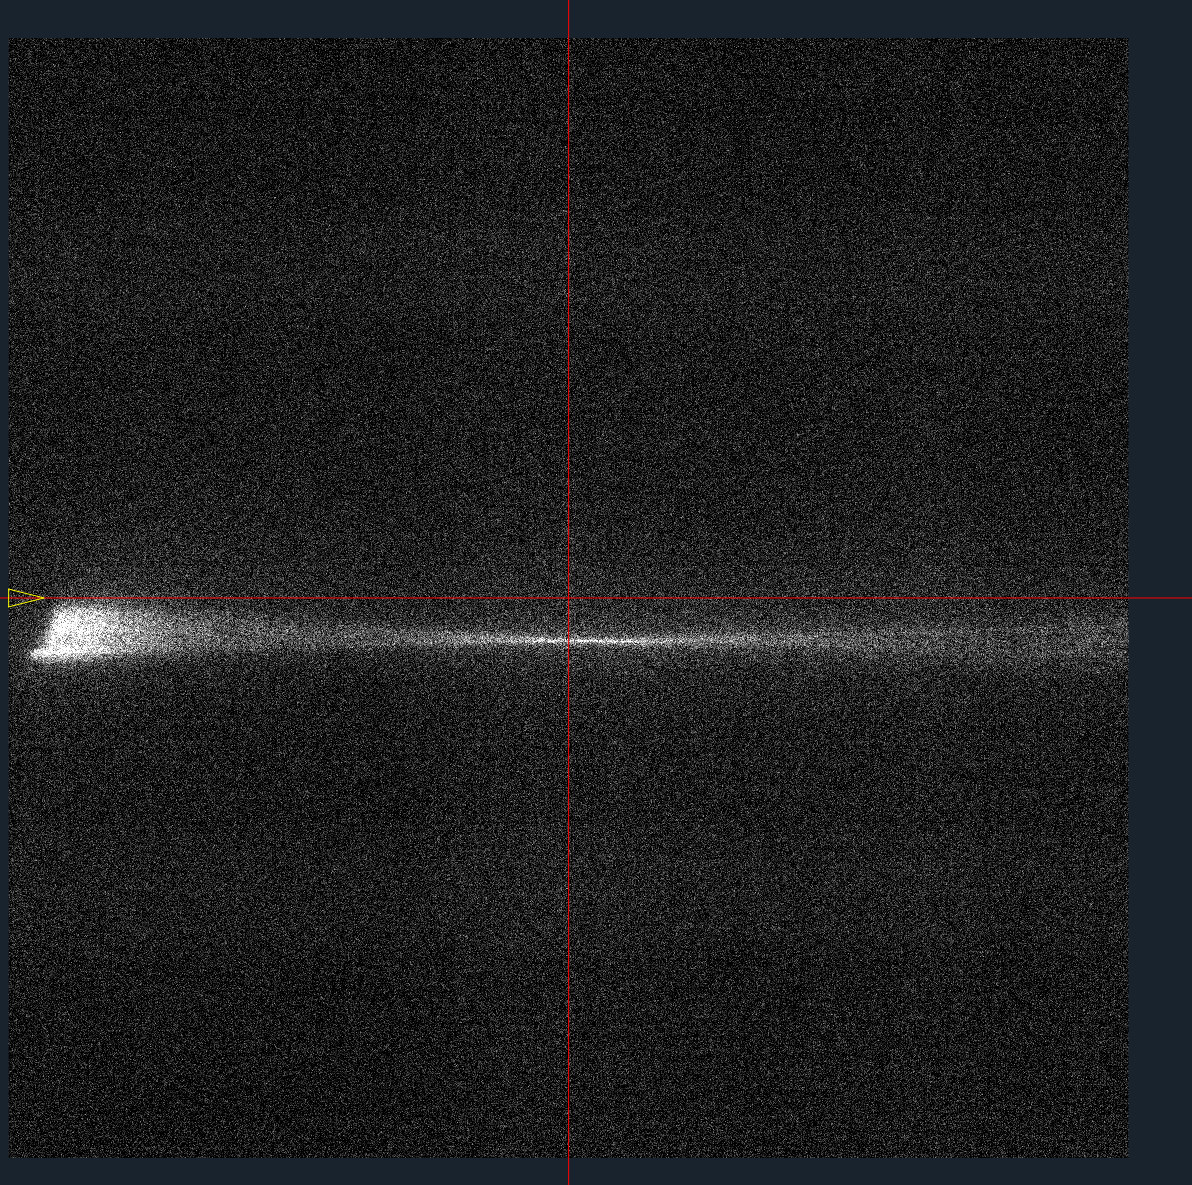
\includegraphics[width=0.9\linewidth]{Images/Ideal_ETL.png}
    \caption{Aligned ETL profile image acquired from camera FOV} 
    \end{subfigure}
    \medskip
    ~    
    \medskip
    \begin{subfigure}[t]{0.4\textwidth}
    \centering
    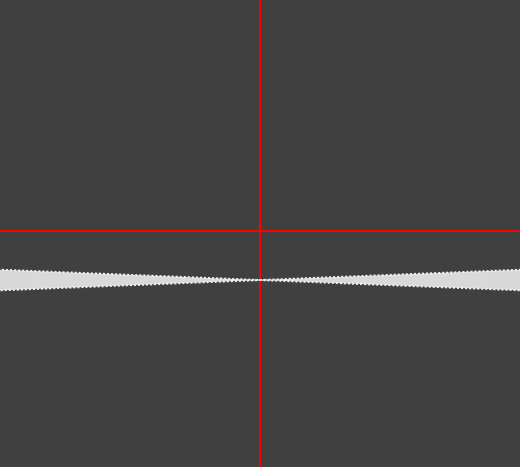
\includegraphics[width=1\linewidth]{Figures/ETL_Profile_TEMP.png}
    \caption{Diagram of aligned ETL profile in camera FOV}
    \end{subfigure}
    \caption{\textbf{Image (a) and diagram (b) of desired offset profile of ETL aligned Gaussian beam in mesoSPIM FOV.} GUI Settings: Galvo mirrors frozen in position, ETL amplitude set to 0.0 V. Digital red line cross hairs mark FOV midlines in mesoSPIM camera feed, replicated in diagram for use in comparing against viewed ETL profile.}
    
\end{figure}

Once both settings are made and this desired beam profile is obtained, the ETL parameters are saved and recorded for future reference. The galvanometer mirrors are unfrozen, and the tissue in the camera FOV is returned to focus, adjusting the position of the objective in increments of 5 µm until the highest resolution of the tissue possible is obtained.

\subsubsection{\textit{Slice Tissue Stack Acquisition}}
To record a .TIFF file of the tissue for data analysis, a custom python code created by Dr. Sharika Mohanan was implemented into the mesoSPIM user interface to allow for imaging of tissue slices oriented at 45 degrees with respect to the detection and excitation pathways. This orientation is required due to the sides of the sample mount obstructing the light sheet when the mount is parallel to the light sheet and obstructing the detection pathway when perpendicular. A copy of the modified python code implemented into the mesoSPIM software to allow for this oblique imaging to proceed can be found in (GITHUB URL HERE). Details regarding the experimental development, processing methodology, and characterization of images acquired using this angled orientation imaging protocol is provided in Chapter 4.2.2-3.

To activate this specialized imaging protocol, a custom ‘Oblique Scanning’ section of the main control page was added to the GUI to activate the angled imaging protocol automatically with no additional insertion of script required from me. For sliced tissues that require oblique scanning throughout the imaged volume, the 'neg 45' check mark box is checked in the 'oblique scanning' custom section. A diagram showing the 'neg 45' mount orientation with respect to the detection and excitation pathways is shown in Figure 2.9.

\begin{figure}[H]
    \centering
    \begin{subfigure}[a]{0.85\textwidth}
    \centering
    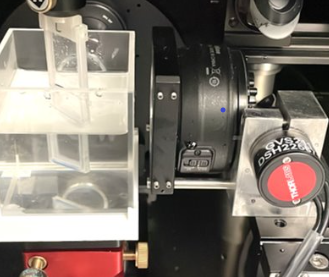
\includegraphics[width=0.85\linewidth]{Figures/Screenshot (168).png}
    \caption{Photo}
    \end{subfigure}
    \medskip
   
    \begin{subfigure}[b]{0.85\textwidth}
    \centering
    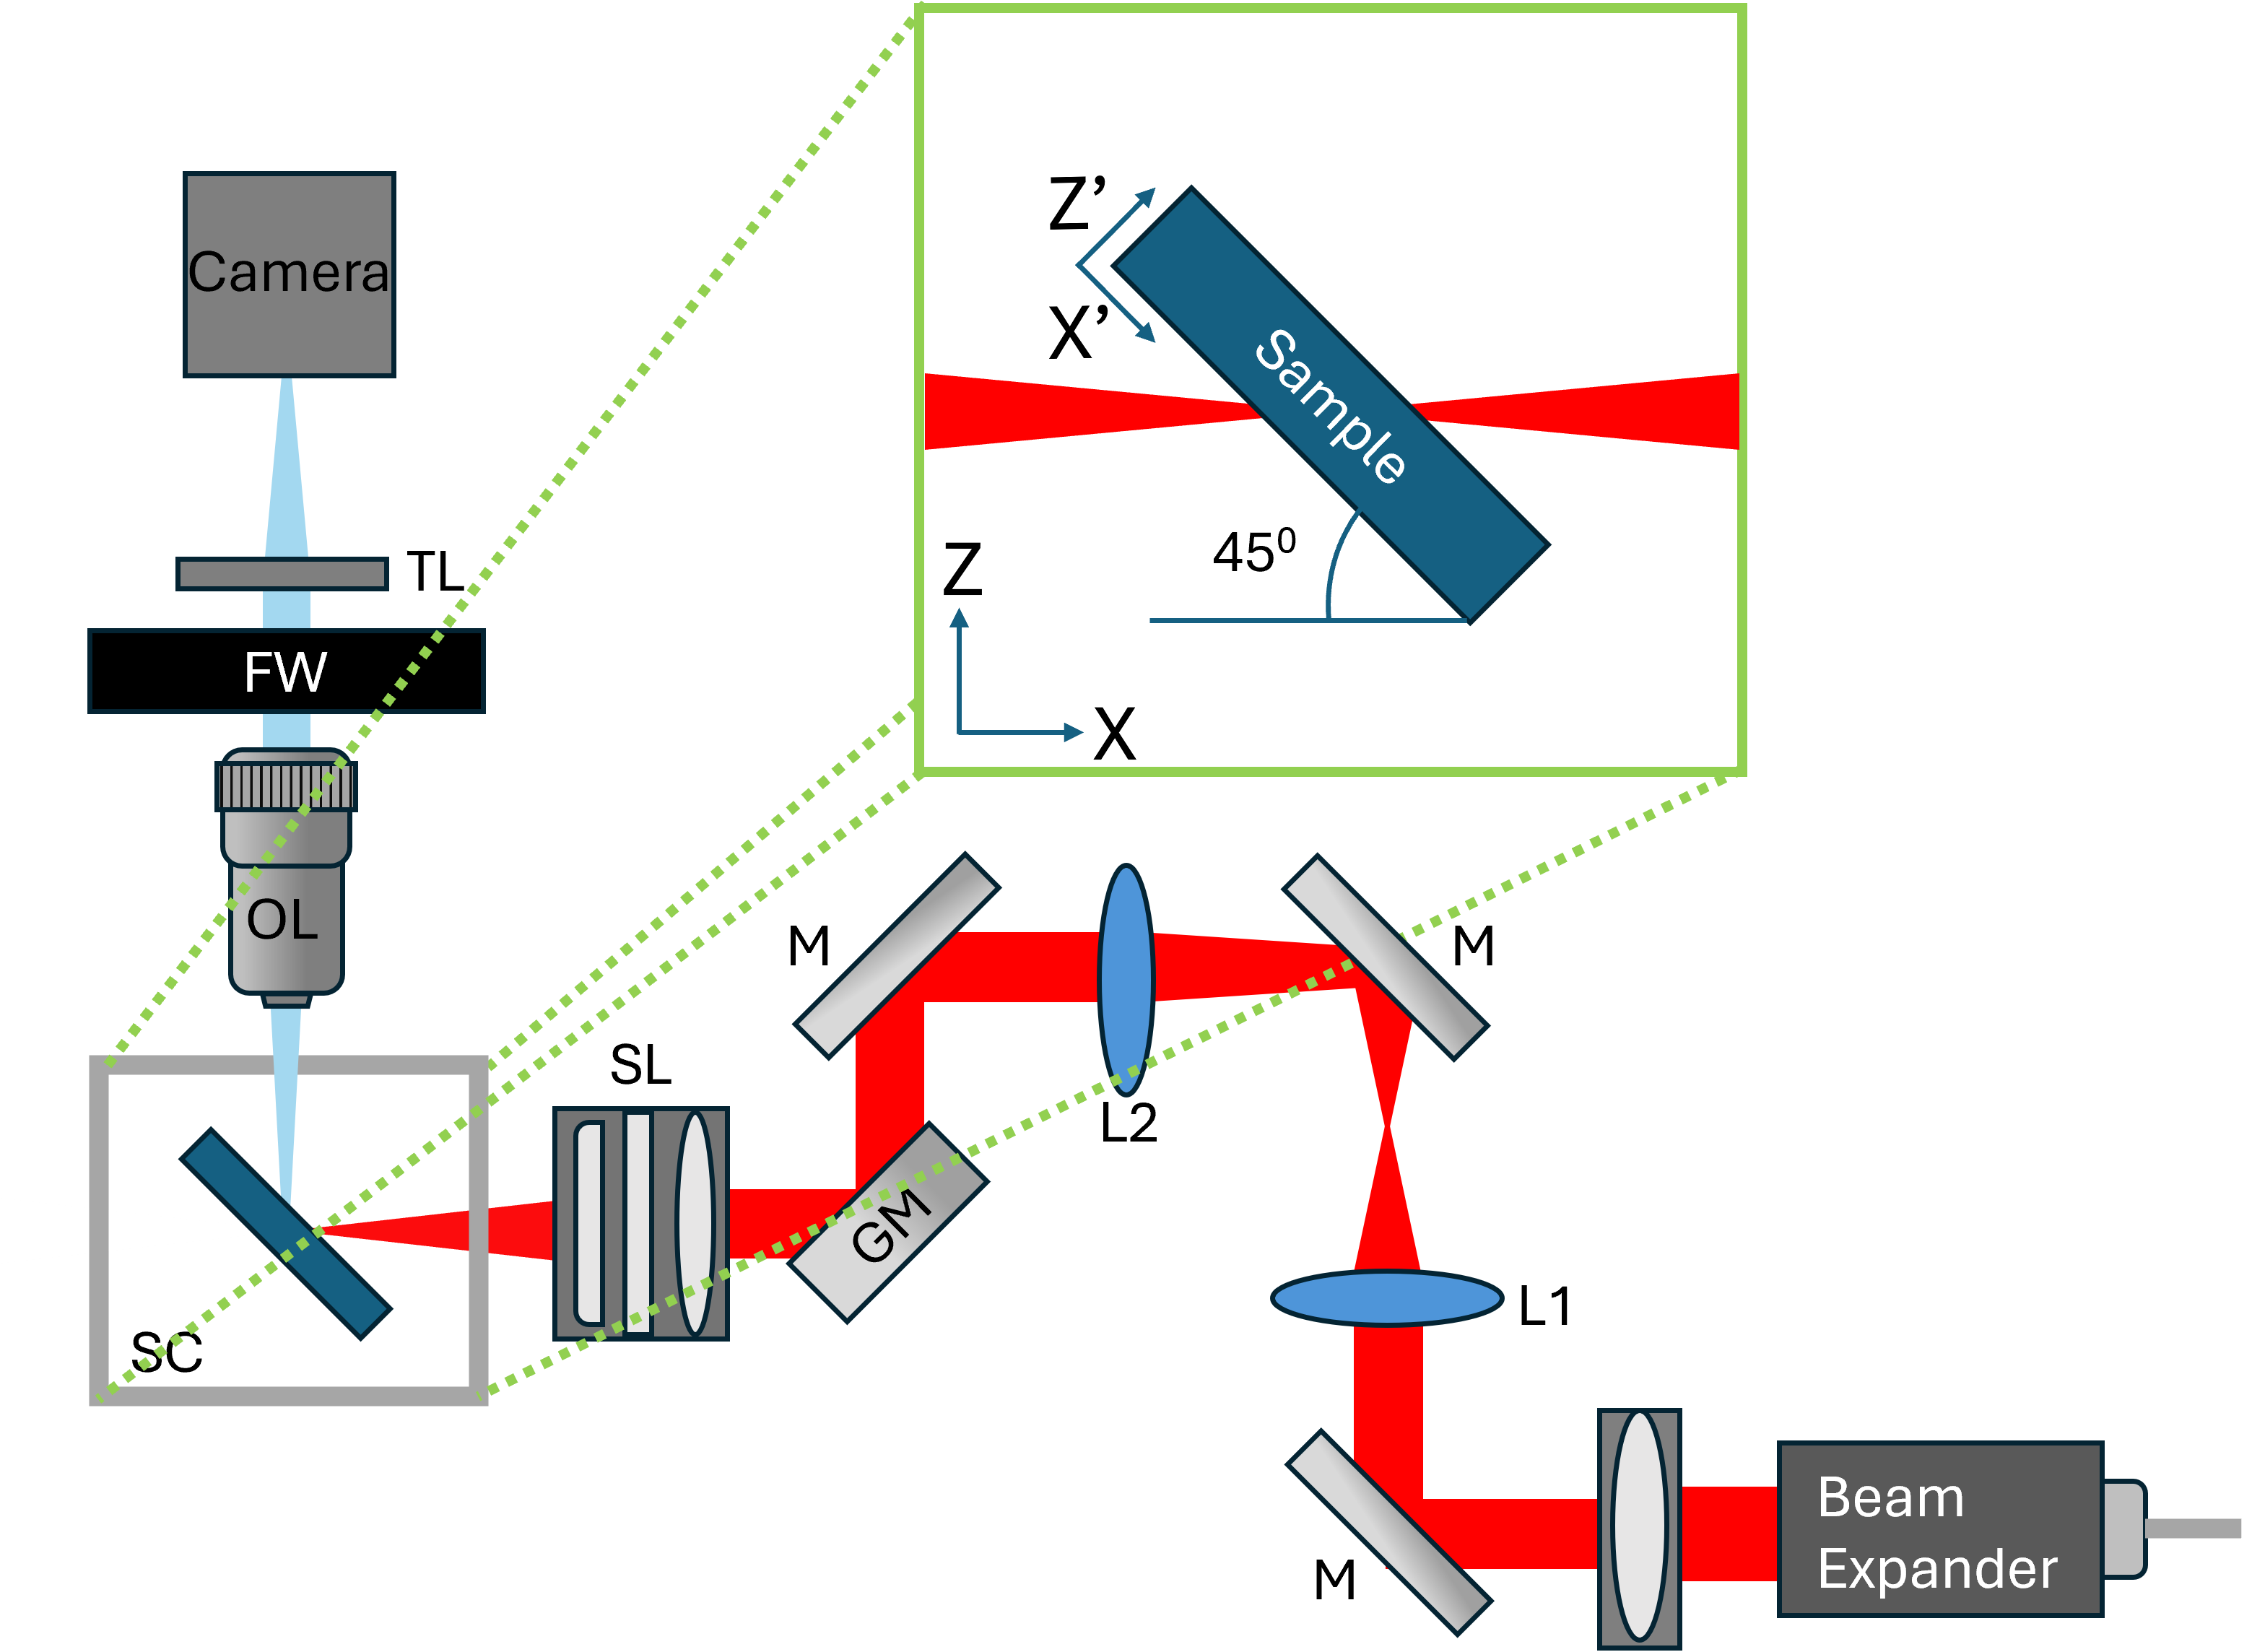
\includegraphics[width=0.85\linewidth]{Figures/Figure2.12.png}
    \caption{Optical Path Diagram (Not to Scale). Legend - ETL: Electronically Tunable Lens; M: Mirrors; L1-2: Lenses; GM: Galvanometer Mirror; SL: Scan Lens; SC: Sample Chamber; OL: Objective Lens; FW: Filter Wheel; TL: Tube Lens.}
    \end{subfigure}
    
    \caption{\textbf{Neg 45 Sample Mounting Orientation.} Photo (a) and Diagram (b) showing excitation, detection pathways relative to mount position.}
    
\end{figure}

The requested parameters required for the acquisition of the stack are shown in a spreadsheet beneath the main control page of the GUI. Here are assigned the acquisition settings, which includes: position of focus stage, laser power, ETL settings, angle orientation of mount, and the start/end positions of the mounted sample in the x,y, and z axes. I adjust these settings in the user interface and views changes in camera view window adjacent to the control window which displays signals captured by the camera in real time. Each setting is set to the optimal values found via manual adjustment of the live camera feed to obtain the highest resolution and contrast image possible of the sample. Y axis movement is kept static for single stack acquisition and z-axis movement is set to 2 microns per frame (~50\% of Axial FWHM, See chapter 4, section 2). The size of the data file and time required to capture all images in this selected stack will be calculated by the mesoSPIM software and displayed once all parameters in a line of the spreadsheet is filled. Parameters are adjusted to accommodate any limitations the connected PC may have in storing large data files (see Section 2.4.3), ensuring the file will not be too large to fit in the drive selected by me to save the data into after acquisition. 

After verifying all selected parameters are accurate and appear in the acquisition spreadsheet and oblique scanning section of the mesoSPIM GUI, the spreadsheet row is highlighted and 'Run Selected Acquisition' is pressed, starting the process of capturing all frames in the designated region of tissue mounted in the system. The system can be left to complete the recording without further human interaction and will return the tissue back to the starting position once completed. The system will display a timer estimating remaining time till imaging is completed which adjusts in real time in accordance to the rolling average speed at which the mesoSPIM captures frames and move the tissue between every camera shutter.


\subsubsection{\textit{Left Ventricle Tissue Tiling Stacks Acquisition}}

To acquire tiling image stacks from a LV tissue sample imaged in the mesoSPIM, a 'Tiling Wizard' program is activated which is included in the mesoSPIM open source software to automatically calculate every position of the sample inside the system that is needs be imaged within a volume designated by me. This volume is determined by me marking the starting and ending coordinated of the volume in the x,y, and z axes. Imaging volumes tiled are programmed to cover the entire tissue sample being imaged with the extrema of the tissue being used to located the x,y, and z coordinates used by the tiling program. I may also specify which combination of laser wavelengths, ETL parameters, and laser power levels will be used in the excitation path as well as which objective, lens filters, and focus settings the system will be at while imaging across the volume. If the focus is set to start and end at different values, the program will increase/decrease the focus value linearly between the starting and end z-axis coordinates. Percentage of FOV overlap between stacks in the tiling protocol can also be set. z-axis movement is set to 3 microns per frame (~50\% of Axial FWHM). For stitching in IMARIS software during post processing, the overlap was kept at default value of 10\% . After verifying all selected parameters appearing in the acquisition spreadsheet are accurate and the oblique scanning section of the mesoSPIM GUI is set to 'zero', all filled spreadsheet rows are highlighted and 'Run Acquisition List' is pressed, starting the process of capturing all tiles in the designated region of tissue mounted in the system. Characterization of images acquired using this imaging protocol will be discussed in Chapter 4.

\subsubsection{\textit{Sliced Tissue Tiling Stack Acquisition}}    

 When setting the starting coordinates for the system 'tiling wizard' program as detailed in the previous section, the 'start' x-axis coordinate is assigned to be equal to the 'end' x-axis coordinate. This keeps the x-axis positioning unchanged for the entire duration of the acquisition process to allow for the oblique scanning process to take place. The remainder of the tiling stack protocol proceeds as detailed in the Left Ventricle Tiling Stacks Acquisition protocol.

\section{Data Processing and Analysis}
\subsection{Fiji ImageJ Software}
Images created for use in presentation of results in this thesis were processed in Fiji ImageJ software \cite{schindelin_fiji_2012}. The software's Brightness and Contrast tool is used to improve visibility of images recorded. Overlapping of image stacks recording identical tissue volumes are also performed using the 'Merge Channels' feature along with the 'Set Scale' and 'Show Scale Bar' features to place all scale bars seen in presented images acquired from the mesoSPIM. 'Histogram', 'Plot Profile', and 'Measure' tools were all utilized to record and plot pixel values across selected regions of interest where required for analysis. Further details regarding the processes utilized to obtain this de-skewed data and experiments conducted to validate their use and accuracy is provided in Chapter 3.

\subsection{Python Data Processing}
Image stacks recorded from samples contained inside 3D printed custom designed mounts and inside internal glass or quartz cuvettes are pre-processed using a python script written by Dr. Sharika Mohanan and Mr. Ahmed Elnageh which restore images back to a 0 degree orientation (if not already recorded at that angle). This script can be found in (GITHUB URL HERE). Further details regarding the processes utilized to obtain this de-skewed data and experiments conducted to validate their use and accuracy is provided in Chapter 4.

\subsection{Oxford Instruments IMARIS Software}
To perform stitching and tiling of large data sets across millimetres of tissue volume, Oxford Instruments IMARIS software was utilized to perform this graphically intensive volume reconstructions \cite{mullan_imaris_nodate,noauthor_imaris_2024}. Discussed here are the protocols established by the IMARIS software developers used to prepare data sets and manipulate them using the software tools and features. Implementation of IMARIS software for data processing and qualitative analysis of large, full volume data sets are provided in Chapter 5.


\subsubsection{\textit{IMARIS File Conversion}}
All \.tif files created for a recorded image stack of LV cardiac tissue sections are loaded onto the IMARIS file converter. Voxel dimensions are set according to the pixel dimensions and magnification of the microscope system used during the recording session This assigns the x and y-axis dimensions  to 1.31 µm x 1.31 µm (at 5x magnification with the camera FOV) and 3 µm for z-axis (50\% the measured axial resolution of system, see Chapter 4.2.3). 

After reading all files, the IMARIS delimiter settings are configured to have F(split) set to match the number of files loaded and all other delimiter options set to 1 (Z,T, etc.). Once set, converter is activated and all files are converted into individual .ims files. IMARIS conversion is performed concurrently on multiple server connected PCs that have the free converter software and is connected to the mesoSPIM PC via Ethernet connection.

\subsubsection{\textit{Tiling Protocol}}
Once all .ims files are created and saved, IMARIS stitcher is opened on an PC with an IMARIS software license All .ims files created from a single wavelength are added to the programme using the 'Add Images' option. 'Position Images on Grid' is then selected from the 'Slice View' submenu to overlap the stacks with 10\% overlap. Grid X, Y values are checked to be accurate to the dimensions of the imaging stacks and image overlapping is checked to be a matching fit between adjacent tiles. Mismatches between tiles are manually adjusted if needed to obtain the best fit between tiles. Once all dimensions and values are confirmed, 'Ok' followed by 'Save' option are selected to save the tiles imaged.   


\subsubsection{\textit{Image Post-Processing}}
Tiled .ims files are opened using the 'Arena' feature of the IMARIS software. Three dimensional analysis is performed by selecting 'ortho slicer' to observe the stack along all orthogonal planes. Secondary and tertiary channels are added to the image by selecting 'Add channel' in the 'Edit' sub-menu. Colours and naming of each channel along with 3D image cropping are achieved using options available in the 'Edit' sub-menu.

Once channels and cropping of tiled image stacks are set, the data is processed using 'Image Proc' with the parameters of processing for each channel selected individually in the sub-window opened by the program. The image processing selection is performed initially on the ROI present in the program's right side sub-window with the results available for preview on the bottom right of the image processing window. Once satisfied with the preview image generated of the ROI, the input values selected for processing of each channel is documented. 'Ok' is then selected in the processing window to perform the processing protocol on the remainder of the three dimensional tiled image. Results are saved for further analysis using ImageJ software and custom Python analysis script.


\subsection{Data Storage and Transfer}
Once Image recording is completed, the mesoSPIM software will create a sub folder containing all stacks and metadata files for each stack recorded. This sub-folder will be sent into the main folder and PC drive specified by me prior to imaging in the acquisitions settings window. Due to the large file sizes of stacks required to image and entire sample (which can be multiple terabytes in size), the files are transferred to a Network Attached Storage (NAS) Device (QNAP TVS-h674T 32GB 6-bay NAS) to allow data to be transferred to other PC systems connected to the same University of Glasgow network as the mesoSPIM system PC.  A diagram showcasing the various data transfers, time durations, storage space size, and drive locations is provided in Figure 2.10.

\begin{figure}[H]
    \centering
    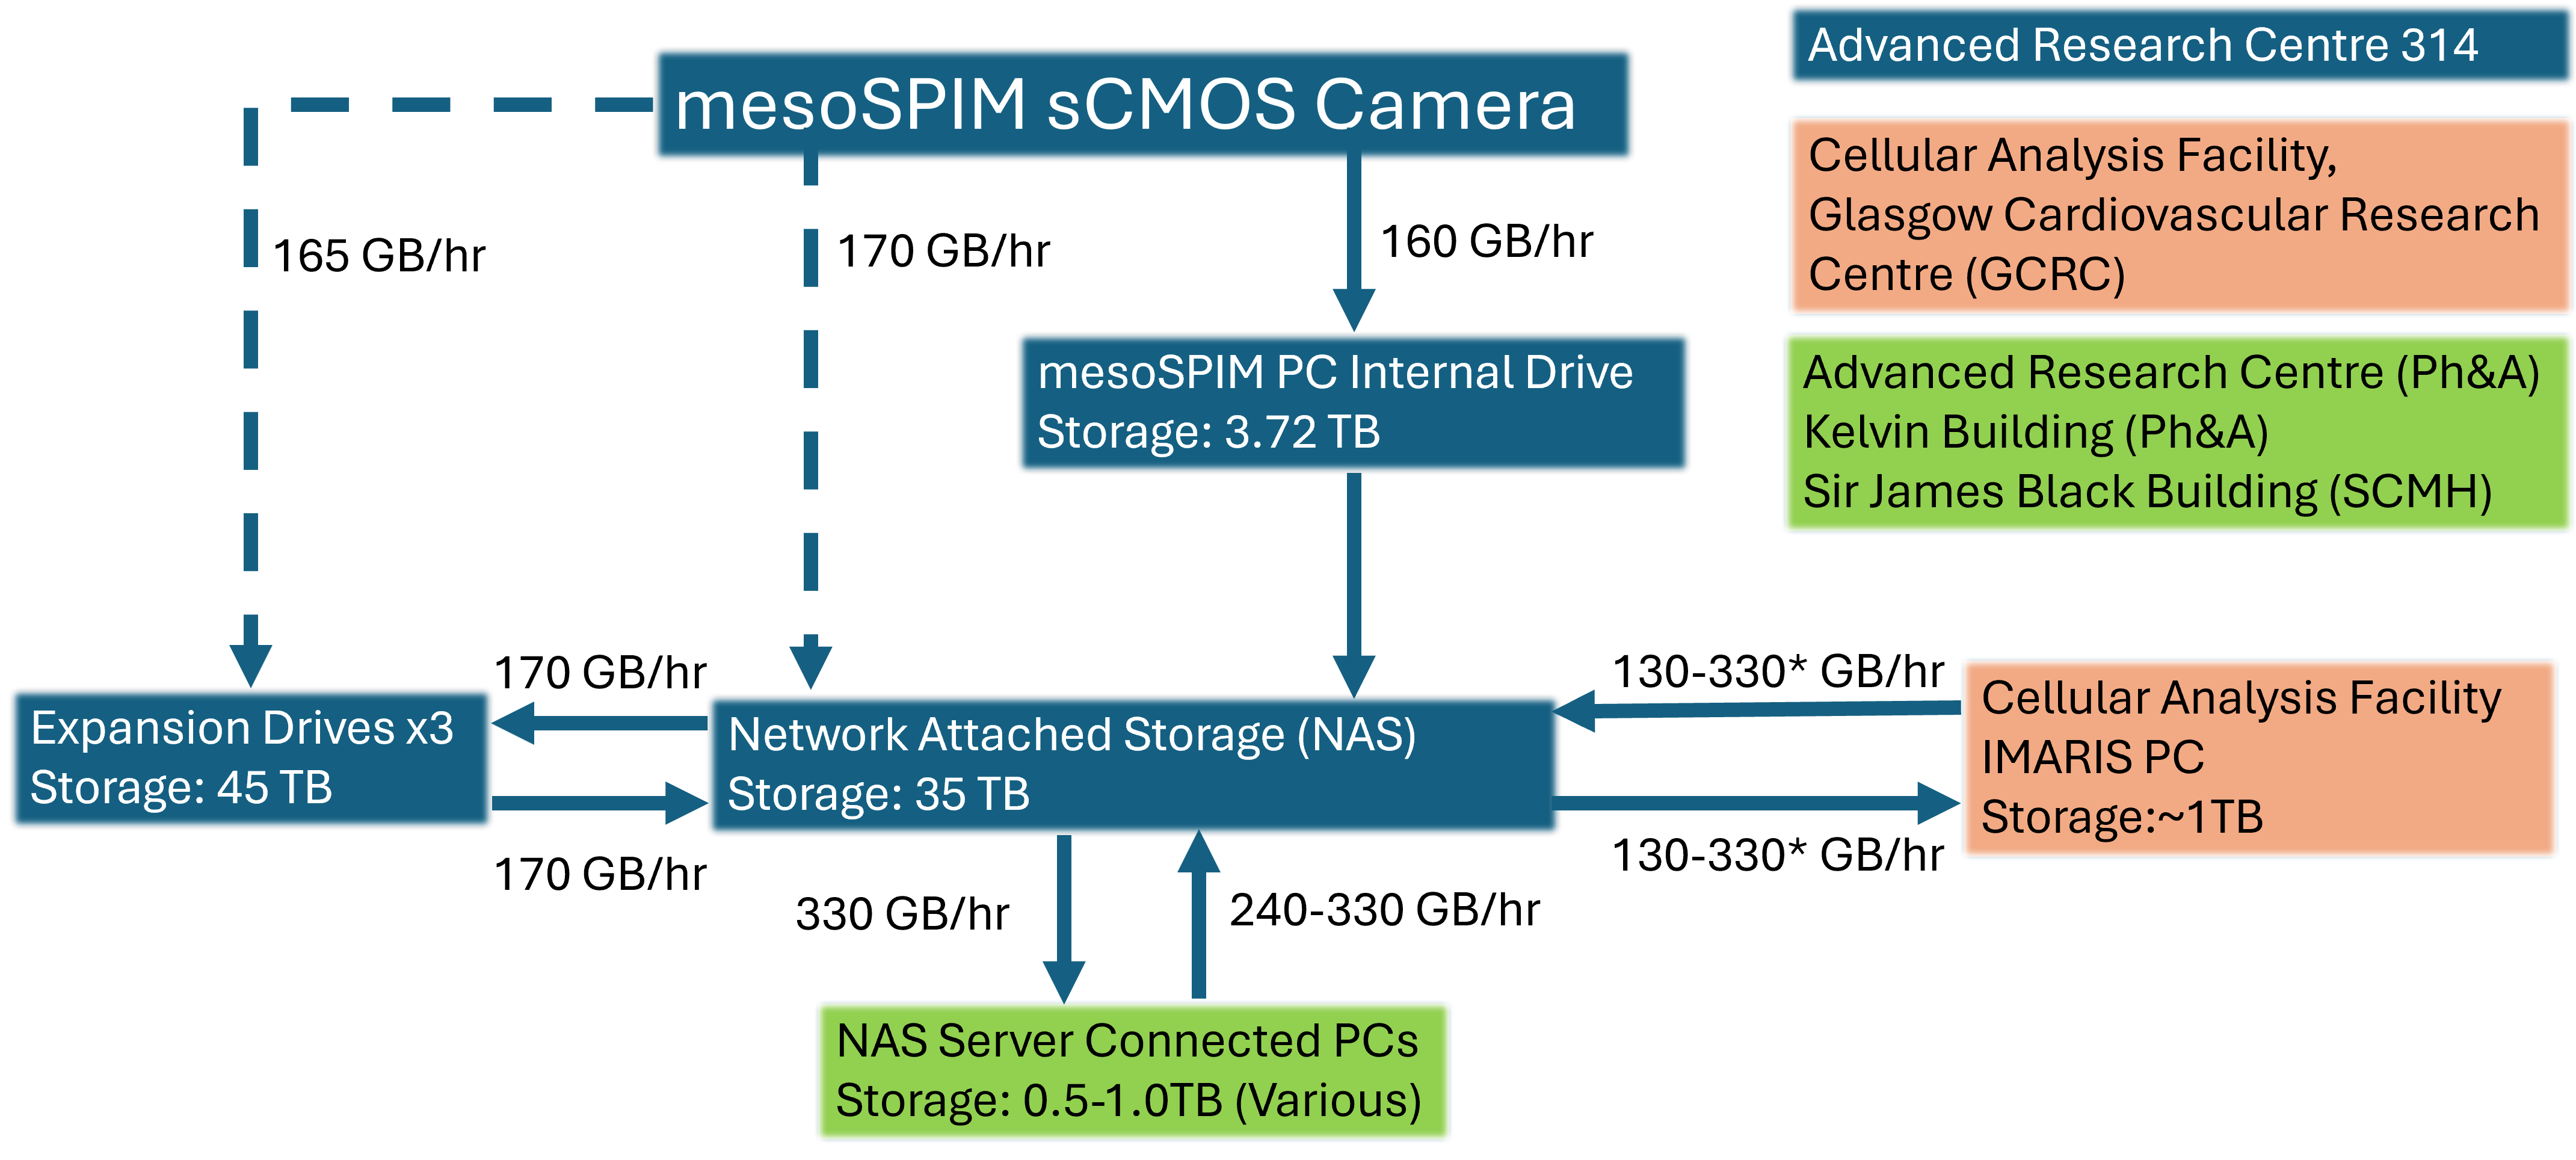
\includegraphics[width=0.95\linewidth]{Figures/Figure2.13TBC.png}
    \caption{\textbf{Diagram of utilized data storage and transfer pathways}. Drive location, transfer speeds, and storage capacities are shown. Dashed pathways: alternative transfer routes bypassing PC internal drive when filled to capacity or in use for unrelated tasks.*Transfer speeds subject to slow down if IMARIS software is in use during transfer.}
    \label{fig:enter-label}
\end{figure}

This established data transfer system allows for ease of access to large data sets for image post-processing, IMARIS file conversions, and subsequent IMARIS tiling and analysis. Due to the limited storage capacity of the NAS, older data sets that have completed post-processing and analysis are transferred over to two separate external hard drives connected to the mesoSPIM control PC for long term data storage and archiving. Transferring data between PC, NAS and external hard drives storage requires multiple hours to complete depending on folder type and size with certain transfer pathways to less powerful PCs requiring even greater lengths of time. Transfers of data are monitored throughout the process to ensure no errors, omissions, or crashes occur during the transfer process. Older data sets are only deleted from the internal PC and NAS drives once it is confirmed all data files in question are: fully transferred to the external drive, not corrupted or improperly formatted, and still accessible for analysis. 

\section{Chapter Summary}
In this chapter, the design and operation of the mesoSPIM LSFM system for implementation into the cardiac tissue imaging pipeline has been explained. It was also demonstrated here that the system's python based GUI can be utilized with specialized mounting and image acquisition coding and procedure to acquire image stacks of mounted, tissue cleared cardiac slices in addition to intact, 3D portions of a cardiac wall. 

Proper and consistent mounting along with custom image acquisition techniques, coding, and settings are essential to the success of subsequent data processing and volumetric image reconstruction of cleared cardiac tissues imaged. The selected volumes images must follow these consistent parameters to recreate the sample volume digitally from the multiple image tiles stitched back together. By integrating custom designed, 3D printed mounts to the existing mesoSPIM design, the system hardware is made compatible for use with fragile slices tissues suspended in RI matching mediums. Customized scripts inserted to the open source python coding of the mesoSPIM GUI allows for the integration of oblique angle imaging of mounted sliced samples into the software's list of control protocols alongside the standard orientation imaging used for non-slice sections of cardiac issue imaged. The subsequent storage and post-processing of this acquired imaging data for use in the final analysis steps of the imaging pipeline was also explored, with emphasis placed on the data storage network created and the software programs and functions utilized to have images sets prepared for use in qualitative and quantitative analysis of tissue structure.

The mesoSPIM system and software programming utilized over the course of this project remains beholden to the condition of the heart tissue inserted into the device for imaging. For the system and subsequent software programmes to produce the desired high fidelity images and volumetric reconstructions of cardiac structure, the tissue must be sufficiently cleared with minimal alteration to the structure. Thus the complete process of achieving and characterizing this crucial tissue clearing step in the imaging pipeline will be the topic covered in the next chapter. 
